% Options for packages loaded elsewhere
\PassOptionsToPackage{unicode}{hyperref}
\PassOptionsToPackage{hyphens}{url}
\PassOptionsToPackage{dvipsnames,svgnames,x11names}{xcolor}
%
\documentclass[
  9pt,
  letterpaper,
]{article}

\usepackage{amsmath,amssymb}
\usepackage{iftex}
\ifPDFTeX
  \usepackage[T1]{fontenc}
  \usepackage[utf8]{inputenc}
  \usepackage{textcomp} % provide euro and other symbols
\else % if luatex or xetex
  \usepackage{unicode-math}
  \defaultfontfeatures{Scale=MatchLowercase}
  \defaultfontfeatures[\rmfamily]{Ligatures=TeX,Scale=1}
\fi
\usepackage{lmodern}
\ifPDFTeX\else  
    % xetex/luatex font selection
\fi
% Use upquote if available, for straight quotes in verbatim environments
\IfFileExists{upquote.sty}{\usepackage{upquote}}{}
\IfFileExists{microtype.sty}{% use microtype if available
  \usepackage[]{microtype}
  \UseMicrotypeSet[protrusion]{basicmath} % disable protrusion for tt fonts
}{}
\makeatletter
\@ifundefined{KOMAClassName}{% if non-KOMA class
  \IfFileExists{parskip.sty}{%
    \usepackage{parskip}
  }{% else
    \setlength{\parindent}{0pt}
    \setlength{\parskip}{6pt plus 2pt minus 1pt}}
}{% if KOMA class
  \KOMAoptions{parskip=half}}
\makeatother
\usepackage{xcolor}
\usepackage[left=20mm,right=20mm,bottom=25mm,top=25mm]{geometry}
\setlength{\emergencystretch}{3em} % prevent overfull lines
\setcounter{secnumdepth}{-\maxdimen} % remove section numbering
% Make \paragraph and \subparagraph free-standing
\makeatletter
\ifx\paragraph\undefined\else
  \let\oldparagraph\paragraph
  \renewcommand{\paragraph}{
    \@ifstar
      \xxxParagraphStar
      \xxxParagraphNoStar
  }
  \newcommand{\xxxParagraphStar}[1]{\oldparagraph*{#1}\mbox{}}
  \newcommand{\xxxParagraphNoStar}[1]{\oldparagraph{#1}\mbox{}}
\fi
\ifx\subparagraph\undefined\else
  \let\oldsubparagraph\subparagraph
  \renewcommand{\subparagraph}{
    \@ifstar
      \xxxSubParagraphStar
      \xxxSubParagraphNoStar
  }
  \newcommand{\xxxSubParagraphStar}[1]{\oldsubparagraph*{#1}\mbox{}}
  \newcommand{\xxxSubParagraphNoStar}[1]{\oldsubparagraph{#1}\mbox{}}
\fi
\makeatother


\providecommand{\tightlist}{%
  \setlength{\itemsep}{0pt}\setlength{\parskip}{0pt}}\usepackage{longtable,booktabs,array}
\usepackage{calc} % for calculating minipage widths
% Correct order of tables after \paragraph or \subparagraph
\usepackage{etoolbox}
\makeatletter
\patchcmd\longtable{\par}{\if@noskipsec\mbox{}\fi\par}{}{}
\makeatother
% Allow footnotes in longtable head/foot
\IfFileExists{footnotehyper.sty}{\usepackage{footnotehyper}}{\usepackage{footnote}}
\makesavenoteenv{longtable}
\usepackage{graphicx}
\makeatletter
\def\maxwidth{\ifdim\Gin@nat@width>\linewidth\linewidth\else\Gin@nat@width\fi}
\def\maxheight{\ifdim\Gin@nat@height>\textheight\textheight\else\Gin@nat@height\fi}
\makeatother
% Scale images if necessary, so that they will not overflow the page
% margins by default, and it is still possible to overwrite the defaults
% using explicit options in \includegraphics[width, height, ...]{}
\setkeys{Gin}{width=\maxwidth,height=\maxheight,keepaspectratio}
% Set default figure placement to htbp
\makeatletter
\def\fps@figure{htbp}
\makeatother
% definitions for citeproc citations
\NewDocumentCommand\citeproctext{}{}
\NewDocumentCommand\citeproc{mm}{%
  \begingroup\def\citeproctext{#2}\cite{#1}\endgroup}
\makeatletter
 % allow citations to break across lines
 \let\@cite@ofmt\@firstofone
 % avoid brackets around text for \cite:
 \def\@biblabel#1{}
 \def\@cite#1#2{{#1\if@tempswa , #2\fi}}
\makeatother
\newlength{\cslhangindent}
\setlength{\cslhangindent}{1.5em}
\newlength{\csllabelwidth}
\setlength{\csllabelwidth}{3em}
\newenvironment{CSLReferences}[2] % #1 hanging-indent, #2 entry-spacing
 {\begin{list}{}{%
  \setlength{\itemindent}{0pt}
  \setlength{\leftmargin}{0pt}
  \setlength{\parsep}{0pt}
  % turn on hanging indent if param 1 is 1
  \ifodd #1
   \setlength{\leftmargin}{\cslhangindent}
   \setlength{\itemindent}{-1\cslhangindent}
  \fi
  % set entry spacing
  \setlength{\itemsep}{#2\baselineskip}}}
 {\end{list}}
\usepackage{calc}
\newcommand{\CSLBlock}[1]{\hfill\break\parbox[t]{\linewidth}{\strut\ignorespaces#1\strut}}
\newcommand{\CSLLeftMargin}[1]{\parbox[t]{\csllabelwidth}{\strut#1\strut}}
\newcommand{\CSLRightInline}[1]{\parbox[t]{\linewidth - \csllabelwidth}{\strut#1\strut}}
\newcommand{\CSLIndent}[1]{\hspace{\cslhangindent}#1}

\usepackage{booktabs}
\usepackage{longtable}
\usepackage{array}
\usepackage{multirow}
\usepackage{wrapfig}
\usepackage{float}
\usepackage{colortbl}
\usepackage{pdflscape}
\usepackage{tabu}
\usepackage{threeparttable}
\usepackage{threeparttablex}
\usepackage[normalem]{ulem}
\usepackage{makecell}
\usepackage{xcolor}
\usepackage[labelfont=bf]{caption}
\makeatletter
\@ifpackageloaded{float}{}{\usepackage{float}}
\floatstyle{plain}
\@ifundefined{c@chapter}{\newfloat{suppfigure}{h}{lofig}}{\newfloat{suppfigure}{h}{lofig}[chapter]}
\floatname{suppfigure}{Figure~S}
\newcommand*\listofsuppfigures{\listof{suppfigure}{List of Figure Ss}}
\makeatother
\makeatletter
\@ifpackageloaded{float}{}{\usepackage{float}}
\floatstyle{plain}
\@ifundefined{c@chapter}{\newfloat{supptbl}{h}{lotbl}}{\newfloat{supptbl}{h}{lotbl}[chapter]}
\floatname{supptbl}{Table~S}
\newcommand*\listofsupptbls{\listof{supptbl}{List of Table Ss}}
\makeatother
\makeatletter
\@ifpackageloaded{caption}{}{\usepackage{caption}}
\AtBeginDocument{%
\ifdefined\contentsname
  \renewcommand*\contentsname{Table of contents}
\else
  \newcommand\contentsname{Table of contents}
\fi
\ifdefined\listfigurename
  \renewcommand*\listfigurename{List of Figures}
\else
  \newcommand\listfigurename{List of Figures}
\fi
\ifdefined\listtablename
  \renewcommand*\listtablename{List of Tables}
\else
  \newcommand\listtablename{List of Tables}
\fi
\ifdefined\figurename
  \renewcommand*\figurename{Figure~S}
\else
  \newcommand\figurename{Figure~S}
\fi
\ifdefined\tablename
  \renewcommand*\tablename{Table~S}
\else
  \newcommand\tablename{Table~S}
\fi
}
\@ifpackageloaded{float}{}{\usepackage{float}}
\floatstyle{ruled}
\@ifundefined{c@chapter}{\newfloat{codelisting}{h}{lop}}{\newfloat{codelisting}{h}{lop}[chapter]}
\floatname{codelisting}{Listing}
\newcommand*\listoflistings{\listof{codelisting}{List of Listings}}
\captionsetup{labelsep=period}
\makeatother
\makeatletter
\makeatother
\makeatletter
\@ifpackageloaded{caption}{}{\usepackage{caption}}
\@ifpackageloaded{subcaption}{}{\usepackage{subcaption}}
\makeatother

\ifLuaTeX
  \usepackage{selnolig}  % disable illegal ligatures
\fi
\usepackage{bookmark}

\IfFileExists{xurl.sty}{\usepackage{xurl}}{} % add URL line breaks if available
\urlstyle{same} % disable monospaced font for URLs
\hypersetup{
  pdftitle={Supplementary Materials for : A matter of size: what underpinned the emergence and demise of the largest rodents that ever lived?},
  pdfauthor={Lucas Buffan¹*, Myriam Boivin\^{}\{2,3\}*, Alicia Álvarez\^{}\{2,3\}, Fabien L. Condamine¹, Laurent Marivaux¹},
  colorlinks=true,
  linkcolor={blue},
  filecolor={Maroon},
  citecolor={Blue},
  urlcolor={Blue},
  pdfcreator={LaTeX via pandoc}}


\title{\emph{Supplementary Materials for} : A matter of size: what
underpinned the emergence and demise of the largest rodents that ever
lived?}
\author{Lucas Buffan¹*, Myriam Boivin\(^{2,3}\)*, Alicia
Álvarez\(^{2,3}\), Fabien L. Condamine¹, Laurent Marivaux¹}
\date{}

\begin{document}
\maketitle


¹ Institut des Sciences de l'Évolution de Montpellier, Université de
Montpellier, CNRS, IRD, Place Eugène Bataillon, 34095 Montpellier cedex
5, France.\\
² Laboratorio de Paleontología de Vertebrados, Instituto de Ecorregiones
Andinas (INECOA), CONICET -- Universidad Nacional de Jujuy, Avenida
Bolivia 1661, 4600 San Salvador de Jujuy, Jujuy, Argentina.\\
³ Instituto de Geología y Minería (IdGyM), Universidad Nacional de
Jujuy, Avenida Bolivia 1661, 4600 San Salvador de Jujuy, Jujuy,
Argentina

* corresponding authors: lucas.l.buffan@gmail.com,
mboivin@idgym.unju.edu.ar

This file contains:

\begin{itemize}
\tightlist
\item
  Supplementary text
\item
  Supplementary figures
\item
  Supplementary tables
\end{itemize}

\hfill\break

Codes are available at:
\url{https://github.com/Buffan3369/Chinchilloids.git}.

Other Supplementary Materials may be found at:
\url{https://doi.org/10.6084/m9.figshare.33111809}.

\newpage

\section{Supplementary text}\label{supplementary-text}

Additional details regarding the cleaning process are provided in the
\texttt{Remark} and \texttt{Age\ justification} columns of \emph{Dataset
S1}.

\subsection{Taxonomic decisions}\label{taxonomic-decisions}

Given that \emph{Lagostomus (Lagostomopsis)} is a subgenus
(\citeproc{ref-rasia2012}{Rasia and Candela 2012}), we set the
\texttt{genus} column of each \emph{Lagostomus (Lagostomopsis)}
occurrence to \emph{Lagostomus}, and switched their
\texttt{genus\_level\_status} from \texttt{extinct} to \texttt{extant}.

All specimens referred to as \emph{Lagostomus cavifrons}, \emph{L.
debilis}, \emph{L. egenus}, \emph{L. heterogenidens} and \emph{L.
minimus} were synonymised with \emph{Lagostomus maximus}, following
(\citeproc{ref-ubilla2016}{Ubilla and Rinderknecht 2016};
\citeproc{ref-rasia_vizcacha_2024}{Rasia 2024}).

Following Busker et al. (\citeproc{ref-busker2019}{2019}), we added two
occurrences of \emph{Saremmys ligcura} from the two localities of Bryn
Gwyn and Gran Barranca (Chubut, Argentina).

We incorporated four occurrences -- corresponding to four different taxa
-- from the AMD-45 locality (18.9--17.1 Ma) published by Arnal et al.
(\citeproc{ref-arnal2026}{2026}): \emph{Maquiamys praecursor},
\emph{Manumys materdei}, \emph{Marianamys altadens} and
\emph{Peruchinchilla prima}.

We followed the latest taxonomic revisions proposed by Rasia
(\citeproc{ref-rasia2026}{2026}) regarding the hyperdiverse dinomyid
fauna from the Ituzaingó Formation (Late Miocene).

\subsection{Age of the
localities/formations}\label{age-of-the-localitiesformations}

The age ranges of the Miocene occurrences from the Río Santa Cruz
(Santacrucian SALMA) were sharpened based on their assigned locality
(\citeproc{ref-arnal2019}{Arnal et al. 2019}). Hence, occurrence from
Barrancas Blancas and Segundas Barrancas Blancas were respectively
assigned the 16.49--17.45 and 15.63--16.46 Ma intervals
(\citeproc{ref-fernicola2019}{Fernicola et al. 2019}).

The single occurrence assigned to \emph{Lagostomus striatus} was removed
as considered \emph{nomen nodum} by Rasia
(\citeproc{ref-rasia2016}{2016}).

The age of the Ituzaingó formation was set to Huayquerian SALMA (Late
Miocene), \emph{ca}. 5--8 Ma (\citeproc{ref-romano2023}{Romano et al.
2023}).

The age range of occurrences from Bucher et al.
(\citeproc{ref-bucher2021}{2021}) were set to the one of the original
publication: 14.6--12.75 Ma when coming from the ``Cruces Infinitos''
and ``Los Yeguarizos localities'', 12.75--12.05 Ma when coming from the
``La Gloria'' and ``La Hoyada'' localities.

Based on Brandoni et al. (\citeproc{ref-brandoni2016}{2016}), the age
range of the occurrences from the Pinturas fauna (\emph{e}.\emph{g}.,
\citeproc{ref-kramarz2002}{Kramarz 2002};
\citeproc{ref-kramarz2004}{2004}; \citeproc{ref-kramarz2006}{2006}),
Burdigalian, were set between 20 and 16.8 Ma.

The age range of the occurrences belonging to the Andalhualá Formation
was set to Huayquerian--Chapadmalalan, \emph{ca}. 7.14--3.66 Ma
(\citeproc{ref-esteban2014}{Esteban et al. 2014};
\citeproc{ref-esteban2019}{2019}).

The age range of the occurrences belonging to the Sierra Baguales (Santa
Cruz formation, Magallanes, Chile) were set to 19--17.8 Ma according to
the isotopic constraints provided in Bostelmann et al.
(\citeproc{ref-bostelmann2013}{2013}).

The age range of the occurrences reported from the Cerro Boleadoras
Formation was set to 16.5--15.1 Ma, according to Vizcaino et al.
(\citeproc{ref-vizcaino2022}{2022}).

\subsection{Remark on extinct chinchilloids from Caribbean
islands}\label{remark-on-extinct-chinchilloids-from-caribbean-islands}

Systematics based on morphological characters {[}primarily dental
traits; Marivaux et al. (\citeproc{ref-marivaux_early_2020}{2020}){]}
also placed the Pleistocene Caribbean `Giant Hutias'
\(\dagger\)\emph{Amblyrhiza inundata} Cope, 1868 and
\(\dagger\)\emph{Elasmodontomys obliquus} Anthony, 1916 within
Chinchilloidea. One might however mention that, as summarised by
Marivaux et al. (\citeproc{ref-marivaux2022}{2022}), the phylogenetic
placement of \(\dagger\)\emph{Elasmodontomys} still represents a real
\emph{conundrum}, with contrasting sources of evidence either suggesting
this taxon to be nested within Chinchilloidea (\emph{e}.\emph{g}.,
\citeproc{ref-marivaux_early_2020}{Marivaux et al. 2020};
\citeproc{ref-marivaux2022}{2022}), Octodontoidea (\emph{e}.\emph{g}.,
\citeproc{ref-woods2021}{Woods et al. 2021}) -- another caviomorph
superfamily -- or to be a morphological intermediate between those two
clades (\emph{i}.\emph{e}., Octochinchilloi, \emph{sensu} Boivin et al.
(\citeproc{ref-boivin2019}{2019})) (\citeproc{ref-macphee2011}{MacPhee
2011}; \citeproc{ref-dacunha2023}{Da Cunha et al. 2023}).

\subsection{Remarks on the extant taxa lacking fossil
record}\label{remarks-on-the-extant-taxa-lacking-fossil-record}

Remains of \emph{Chinchilla chinchilla} and \emph{Lagidium viscacia}
were in fact once reported from an archaeological assemblage, but we
assume their age to be too close to the present to provide useful
information on the time of speciation of the species.

The validity of \emph{Lagidium peruanum} is questionable. The species
indeed appears on the Mammal Diversity Database 2025
(\citeproc{ref-burgin2025}{Burgin et al. 2025}), but is sometimes
regarded as a synonymous of \emph{L. viscaccia}. For practical reasons
(and as it was included in our phylogeny), we decided to keep it for the
rest of our analyses, but this choice does not reflect any taxonomic
decision.

\newpage

\section{Supplementary Figures}\label{supplementary-figures}

\begin{suppfigure}[H]

\centering{

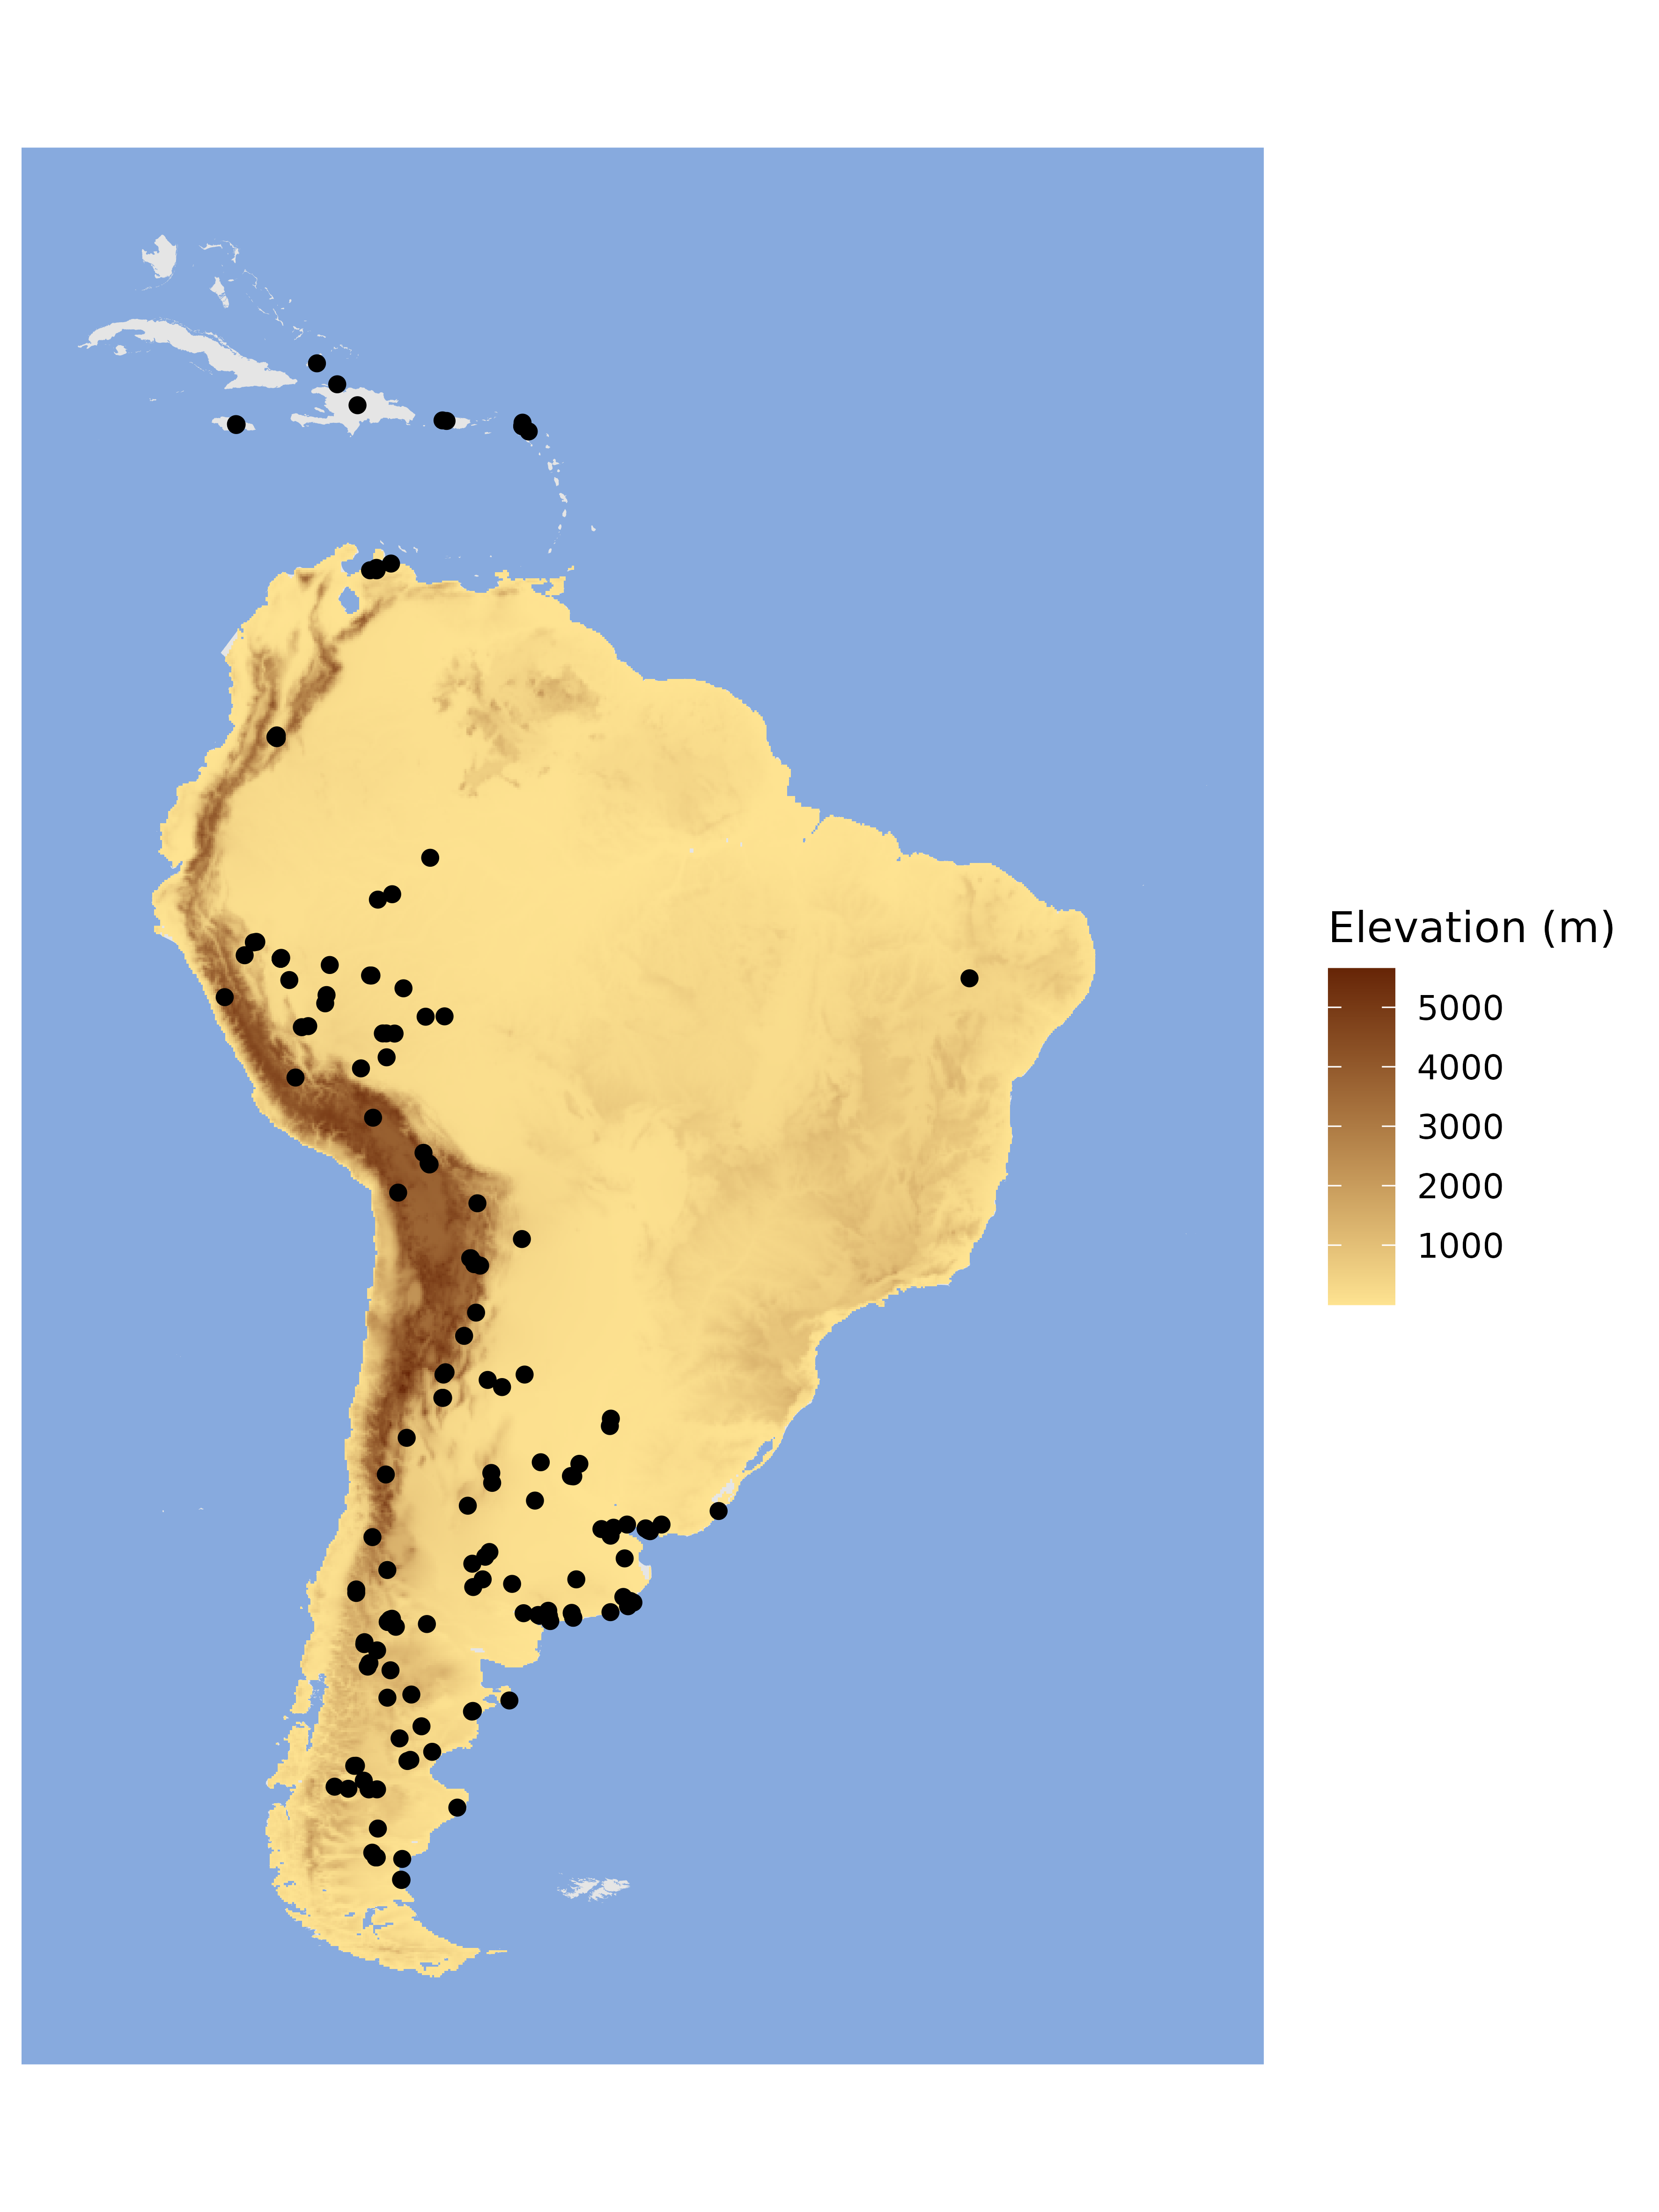
\includegraphics[width=16cm,height=\textheight]{../../Figures/Supp/Occurrence_map_Chinchilloidea.png}

}

\caption{\label{fig-OccMap}Location of the chinchilloid-bearing sites
that yielded the material used in this study (\(N=177\), but note that
some localities have been amalgamated for visual purpose). GPS
coordinates are from The Paleobiology Database.}

\end{suppfigure}%

\begin{suppfigure}[H]

\centering{

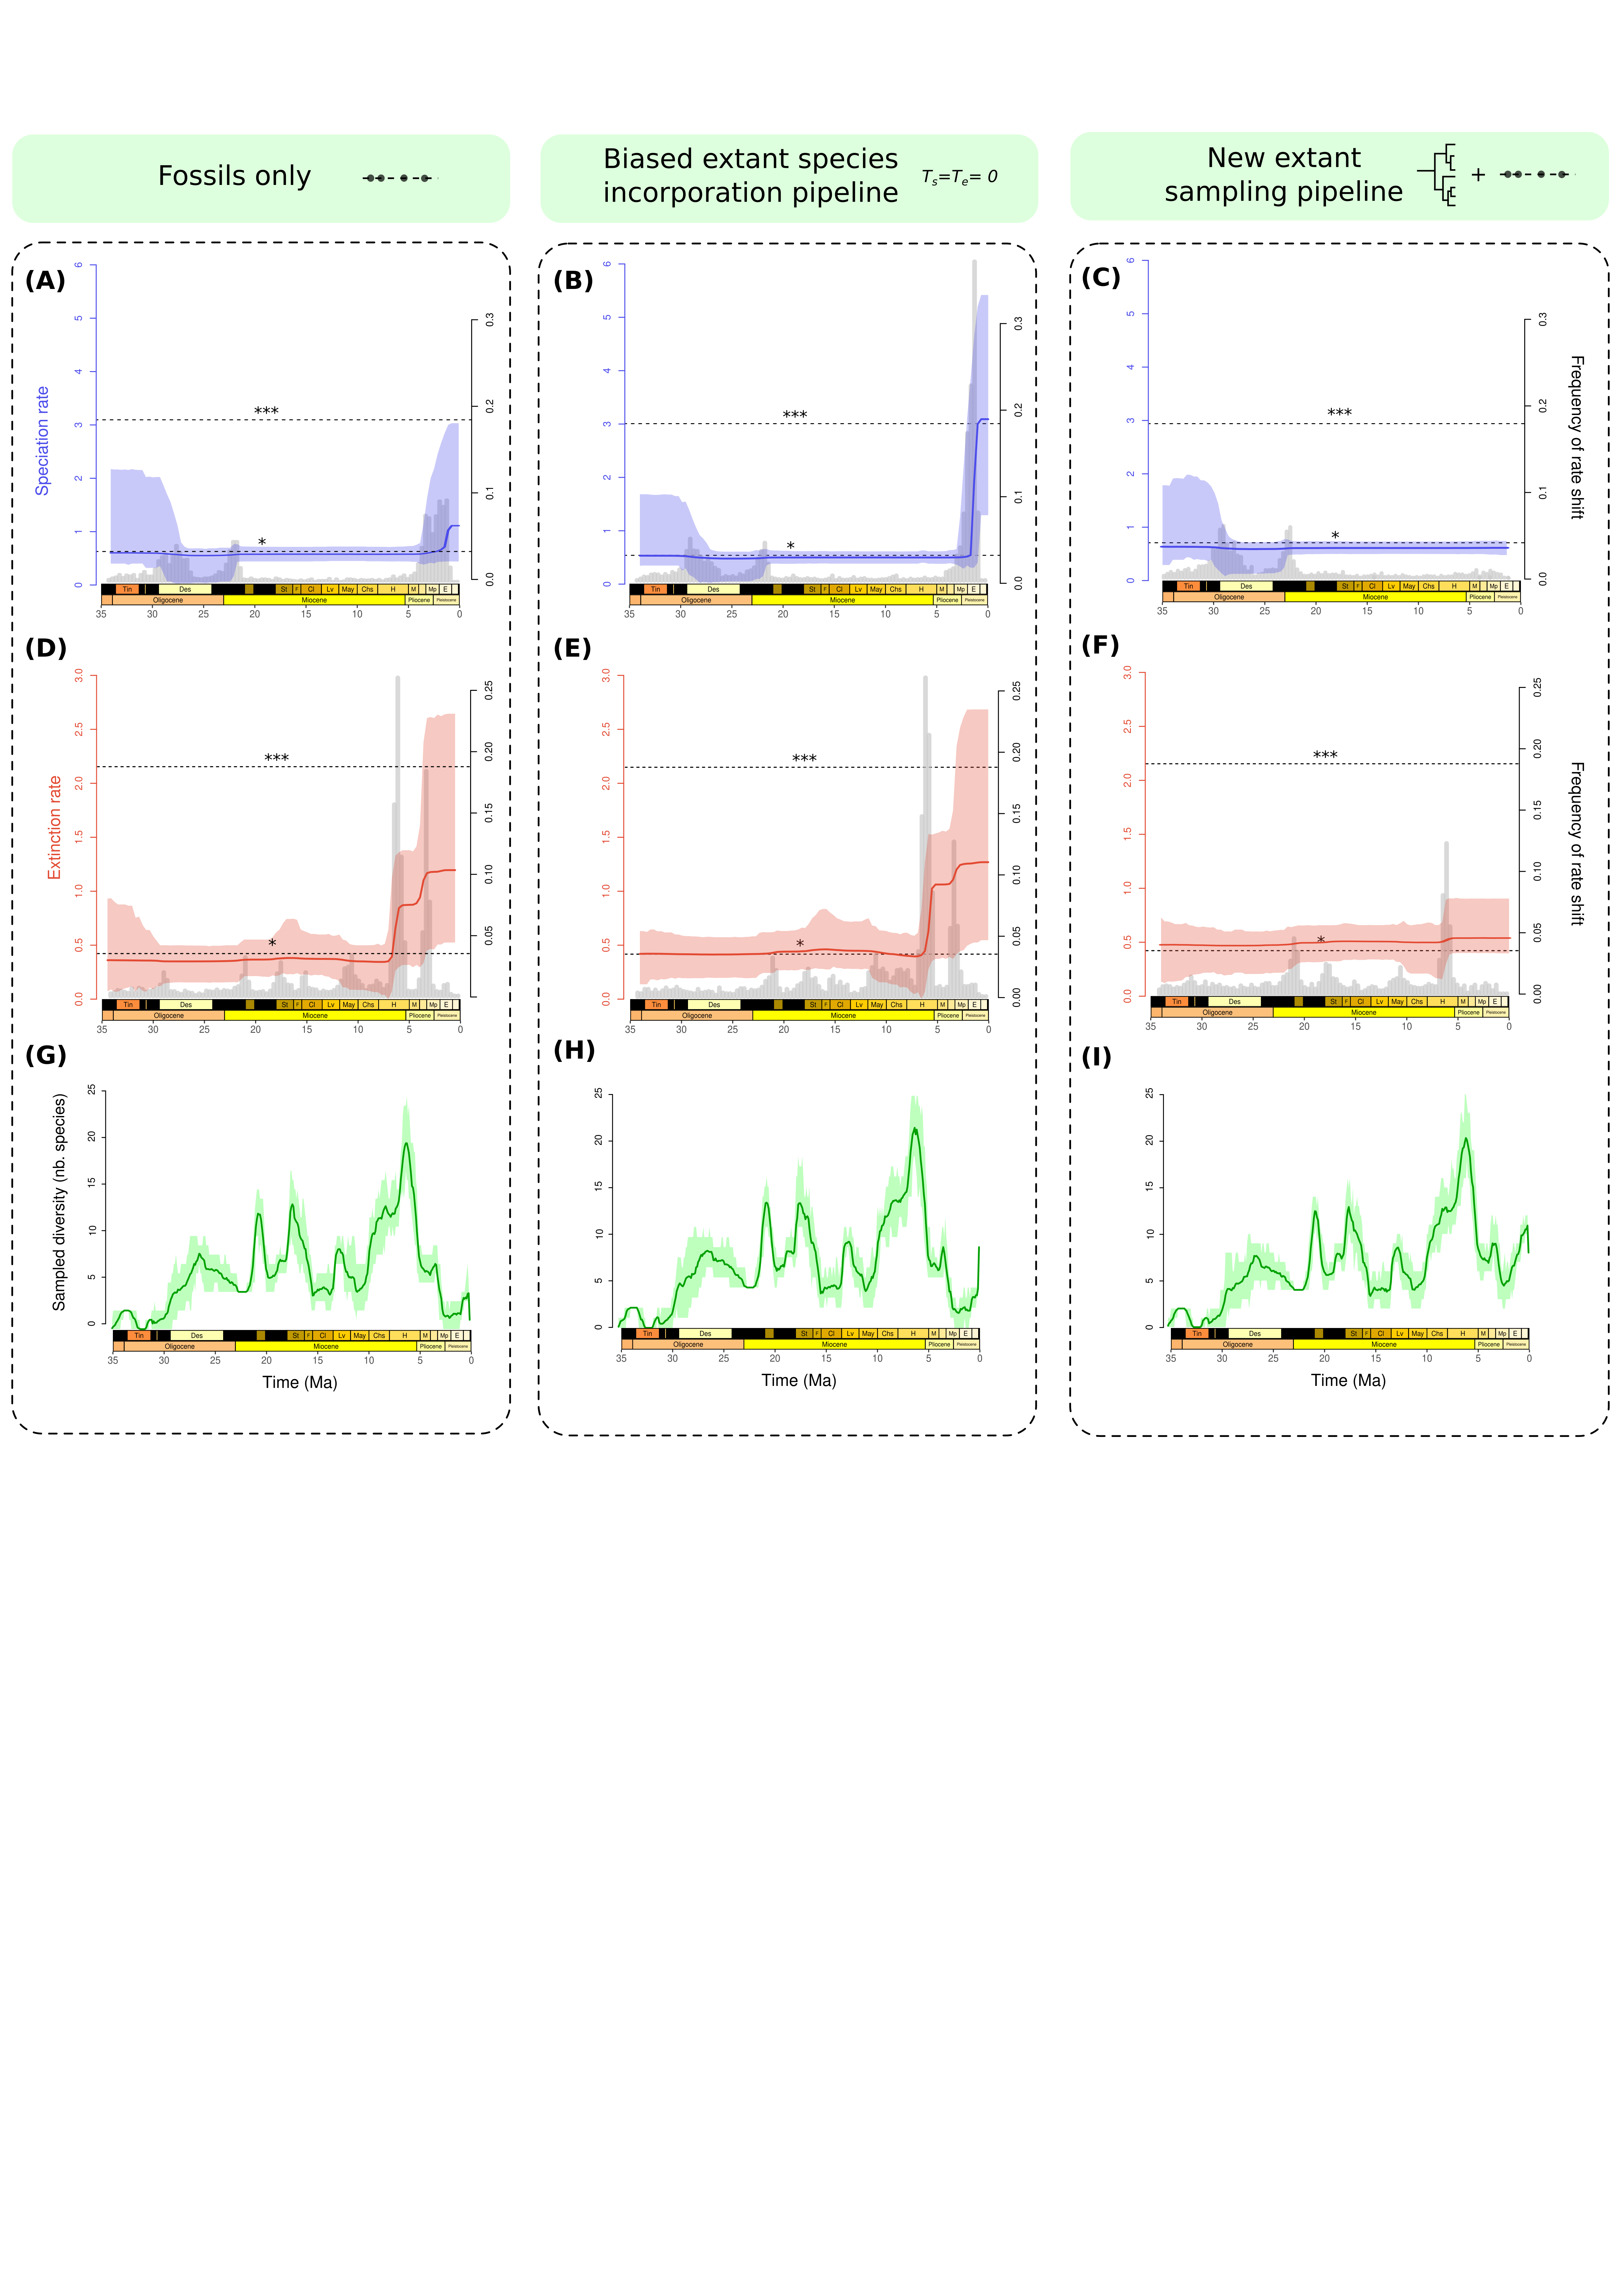
\includegraphics[width=17.5cm,height=\textheight]{../../Figures/Supp/Age_combination_effect/age_comb_effect_RTT.png}

}

\caption{\label{fig-EffectSamplingRTT}Impact of the sampling scheme of
extant species lacking fossil record on upstream macroevolutionary
inferences with PyRate (rjMCMC algorithm). (\textbf{A}, \textbf{D},
\textbf{G}) show speciation rate, extinction rate and sampled diversity
estimated from a database only encompassing fossil taxa. In (\textbf{B},
\textbf{E}, \textbf{H}), extant taxa were included by means of an
occurrence with origination and extinction ages (\(T_e\) and \(T_e\))
set to 0 Ma (\emph{i}.\emph{e}., `biased incorporation'). In
(\textbf{C}, \textbf{F}, \textbf{I}), extant taxa were included or with
our newly-introduced pipeline relying on ages extracted from dated
phylogenies. Full lines indicate median rate estimation (blue for
speciation, \textbf{A}--\textbf{C}, red for extinction,
\textbf{D}--\textbf{F}), and ribbons their associated 95\% HPD interval.
Grey histograms in the background depict the frequency of rate shift per
1-My time bins (\textbf{A}--\textbf{F}). The two horizontal lines
labelled * and *** respectively indicate significant and strongly
supported rate shift (\textbf{A}--\textbf{F}).}

\end{suppfigure}%

\begin{suppfigure}[H]

\centering{

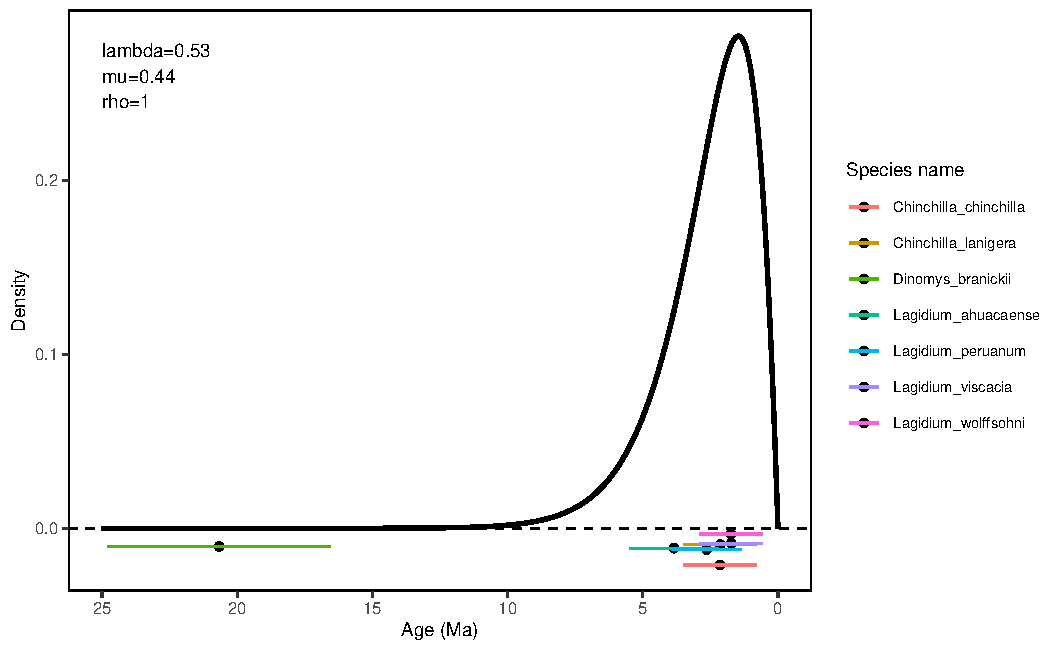
\includegraphics{../../Figures/Supp/ExtantSampling/ExpectedTsDensity.pdf}

}

\caption{\label{fig-TsPhyloPyRate}Expected distribution of the corrected
age of extant taxa from a phylogeny matching our chinchilloid tree in
terms of speciation (`lambda'), extinction rate (`mu') and extant
sampling fraction (`rho'). `lambda' and `mu' were chosen as the basal
extinction and speciation rate values, \emph{i}.\emph{e}., before the
late Miocene change in extinction regime reported in this study (Figure
5 and Figure~S\ref{fig-EffectSamplingRTT}). Dots (along with errorbars)
represent extant chinchilloid species phylogenetic ages (and their 95\%
HPD), extracted from the phylogenetic reconstruction used across this
study (see Main Text, \emph{Methods} section).}

\end{suppfigure}%

\begin{suppfigure}[H]

\centering{

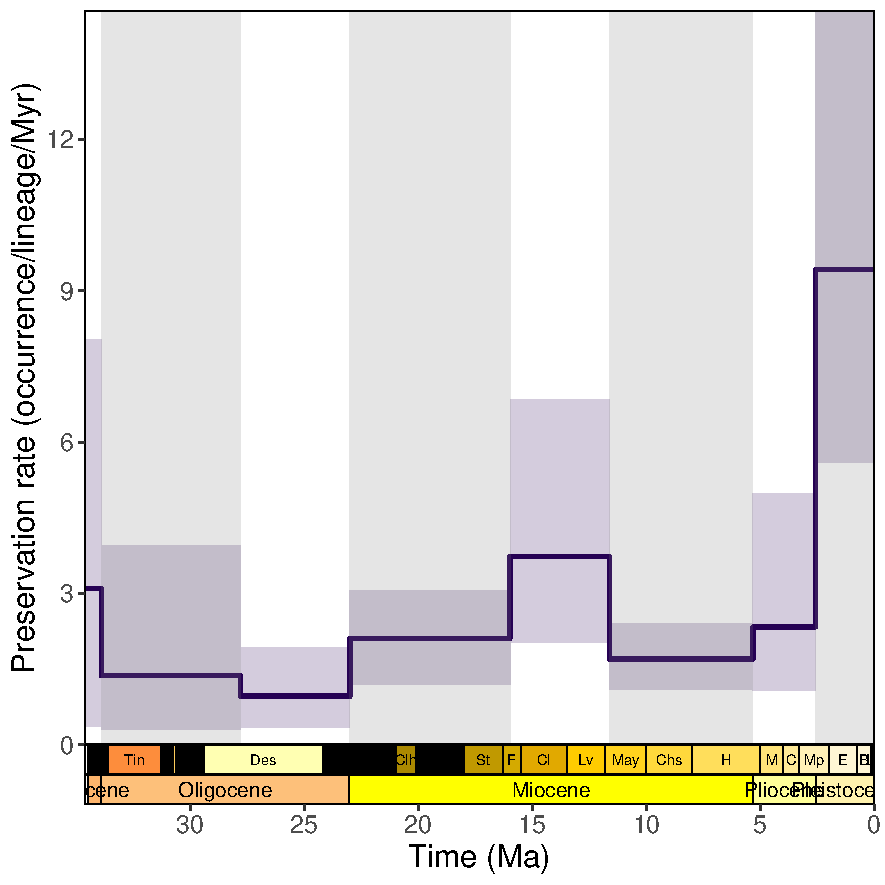
\includegraphics[width=\textwidth,height=9cm]{../../Figures/Supp/Preservation_through_time.pdf}

}

\caption{\label{fig-preservation_rate}Preservation rate through time in
our species-level dataset estimated with PyRate. The solid line
represents the mean posterior estimate and the shaded area the
associated 95\% HPD interval.}

\end{suppfigure}%

\begin{suppfigure}[H]

\centering{

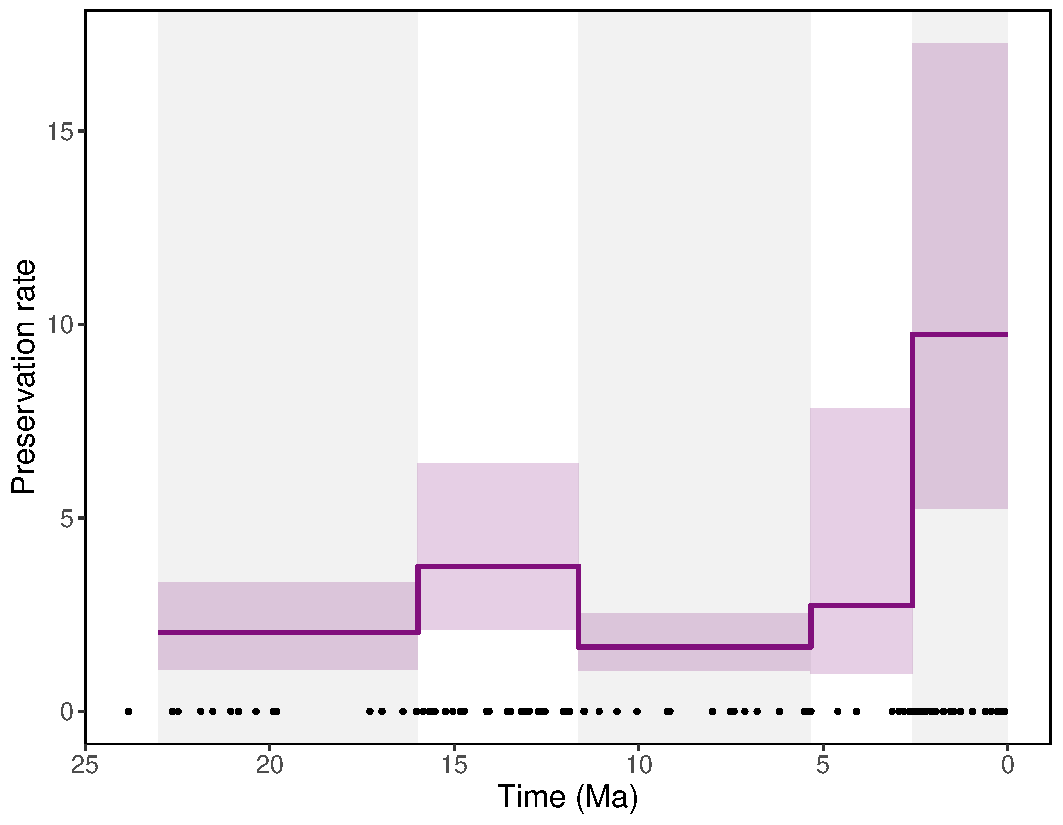
\includegraphics[width=\textwidth,height=9cm]{../../Figures/Supp/ExtantSampling/sampling_plot.pdf}

}

\caption{\label{fig-sampling_scheme}Illustration of our occurrence
sampling pipeline following a Poisson process with piecewise-constant
intensity. The purple line shows the mean posterior preservation rate
obtained from our PyRate fossil-only analyses, and the ribbon its 95\%
HPD interval. Within each preservation rate bin, the intensity of the
occurrence sampling process sas sampled from the posterior distribution
of the preservation rate. Black dots represent sampled occurrences,
along with their sampling times.}

\end{suppfigure}%

\begin{suppfigure}[H]

\centering{

\includegraphics[width=8in,height=8cm]{../../Results/RJMCMC/species/1-Full/pyrate_mcmc_logs/ESS_plot.png}

}

\caption{\label{fig-ESSplot}Convergence of the PyRate runs (rjMCMC
algorithm) for the analysis of the species-level temporal occurrence
database. (\textbf{A}) shows the ESS of the model posterior probability
for all the 20 replicates we ran. ESS greater than 200 (first-scale
indicator of a run that converged, \(n=20\) in that case) are displayed
in green. The yellow and red line respectively depict ESS=200 and
ESS=100. The proportion of origination and extinction times (resp.
\(T_S\) and \(T_E\)) that converged (i.e., with \(ESS > 200\)) are shown
in (\textbf{B}), for each of our 20 replicates. (\textbf{C}) shows the
posterior estimates of the mean root age of our group, together with
their lower and upper boundaries of the 95\% HPD interval, across the 20
replicates.}

\end{suppfigure}%

\begin{suppfigure}[H]

\centering{

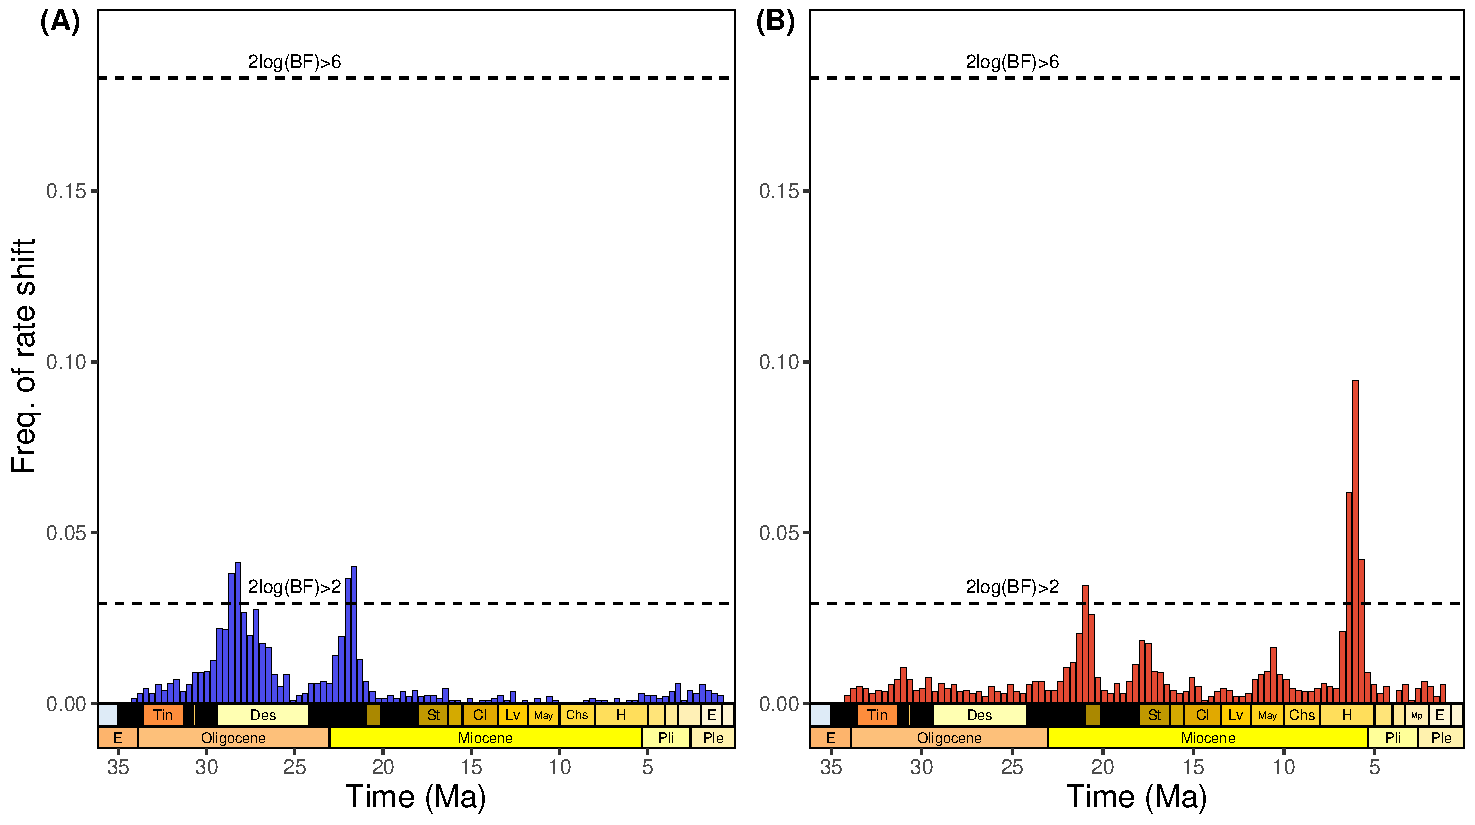
\includegraphics[width=\textwidth,height=8cm]{../../Figures/recap_figures_RJMCMC/New/Chinchilloidea_species_Full_frequency_of_rate_shift.pdf}

}

\caption{\label{fig-FreqRateShift}Histogram showing the frequency of
speciation (\textbf{A}) and extinction (\textbf{B}) rate shifts in our
species-level chinchilloid dataset estimated by PyRate (rjMCMC
algorithm). This quantity indicates, within 1My time bins, the support
given to a model with rate shift compared to a model with constant
rates. The two dashed lines respectively labelled \(2log(BF)>2\) and
\(2log(BF)>6\) respectively indicate significant and strongly supported
rate shift.}

\end{suppfigure}%

\begin{suppfigure}[H]

\centering{

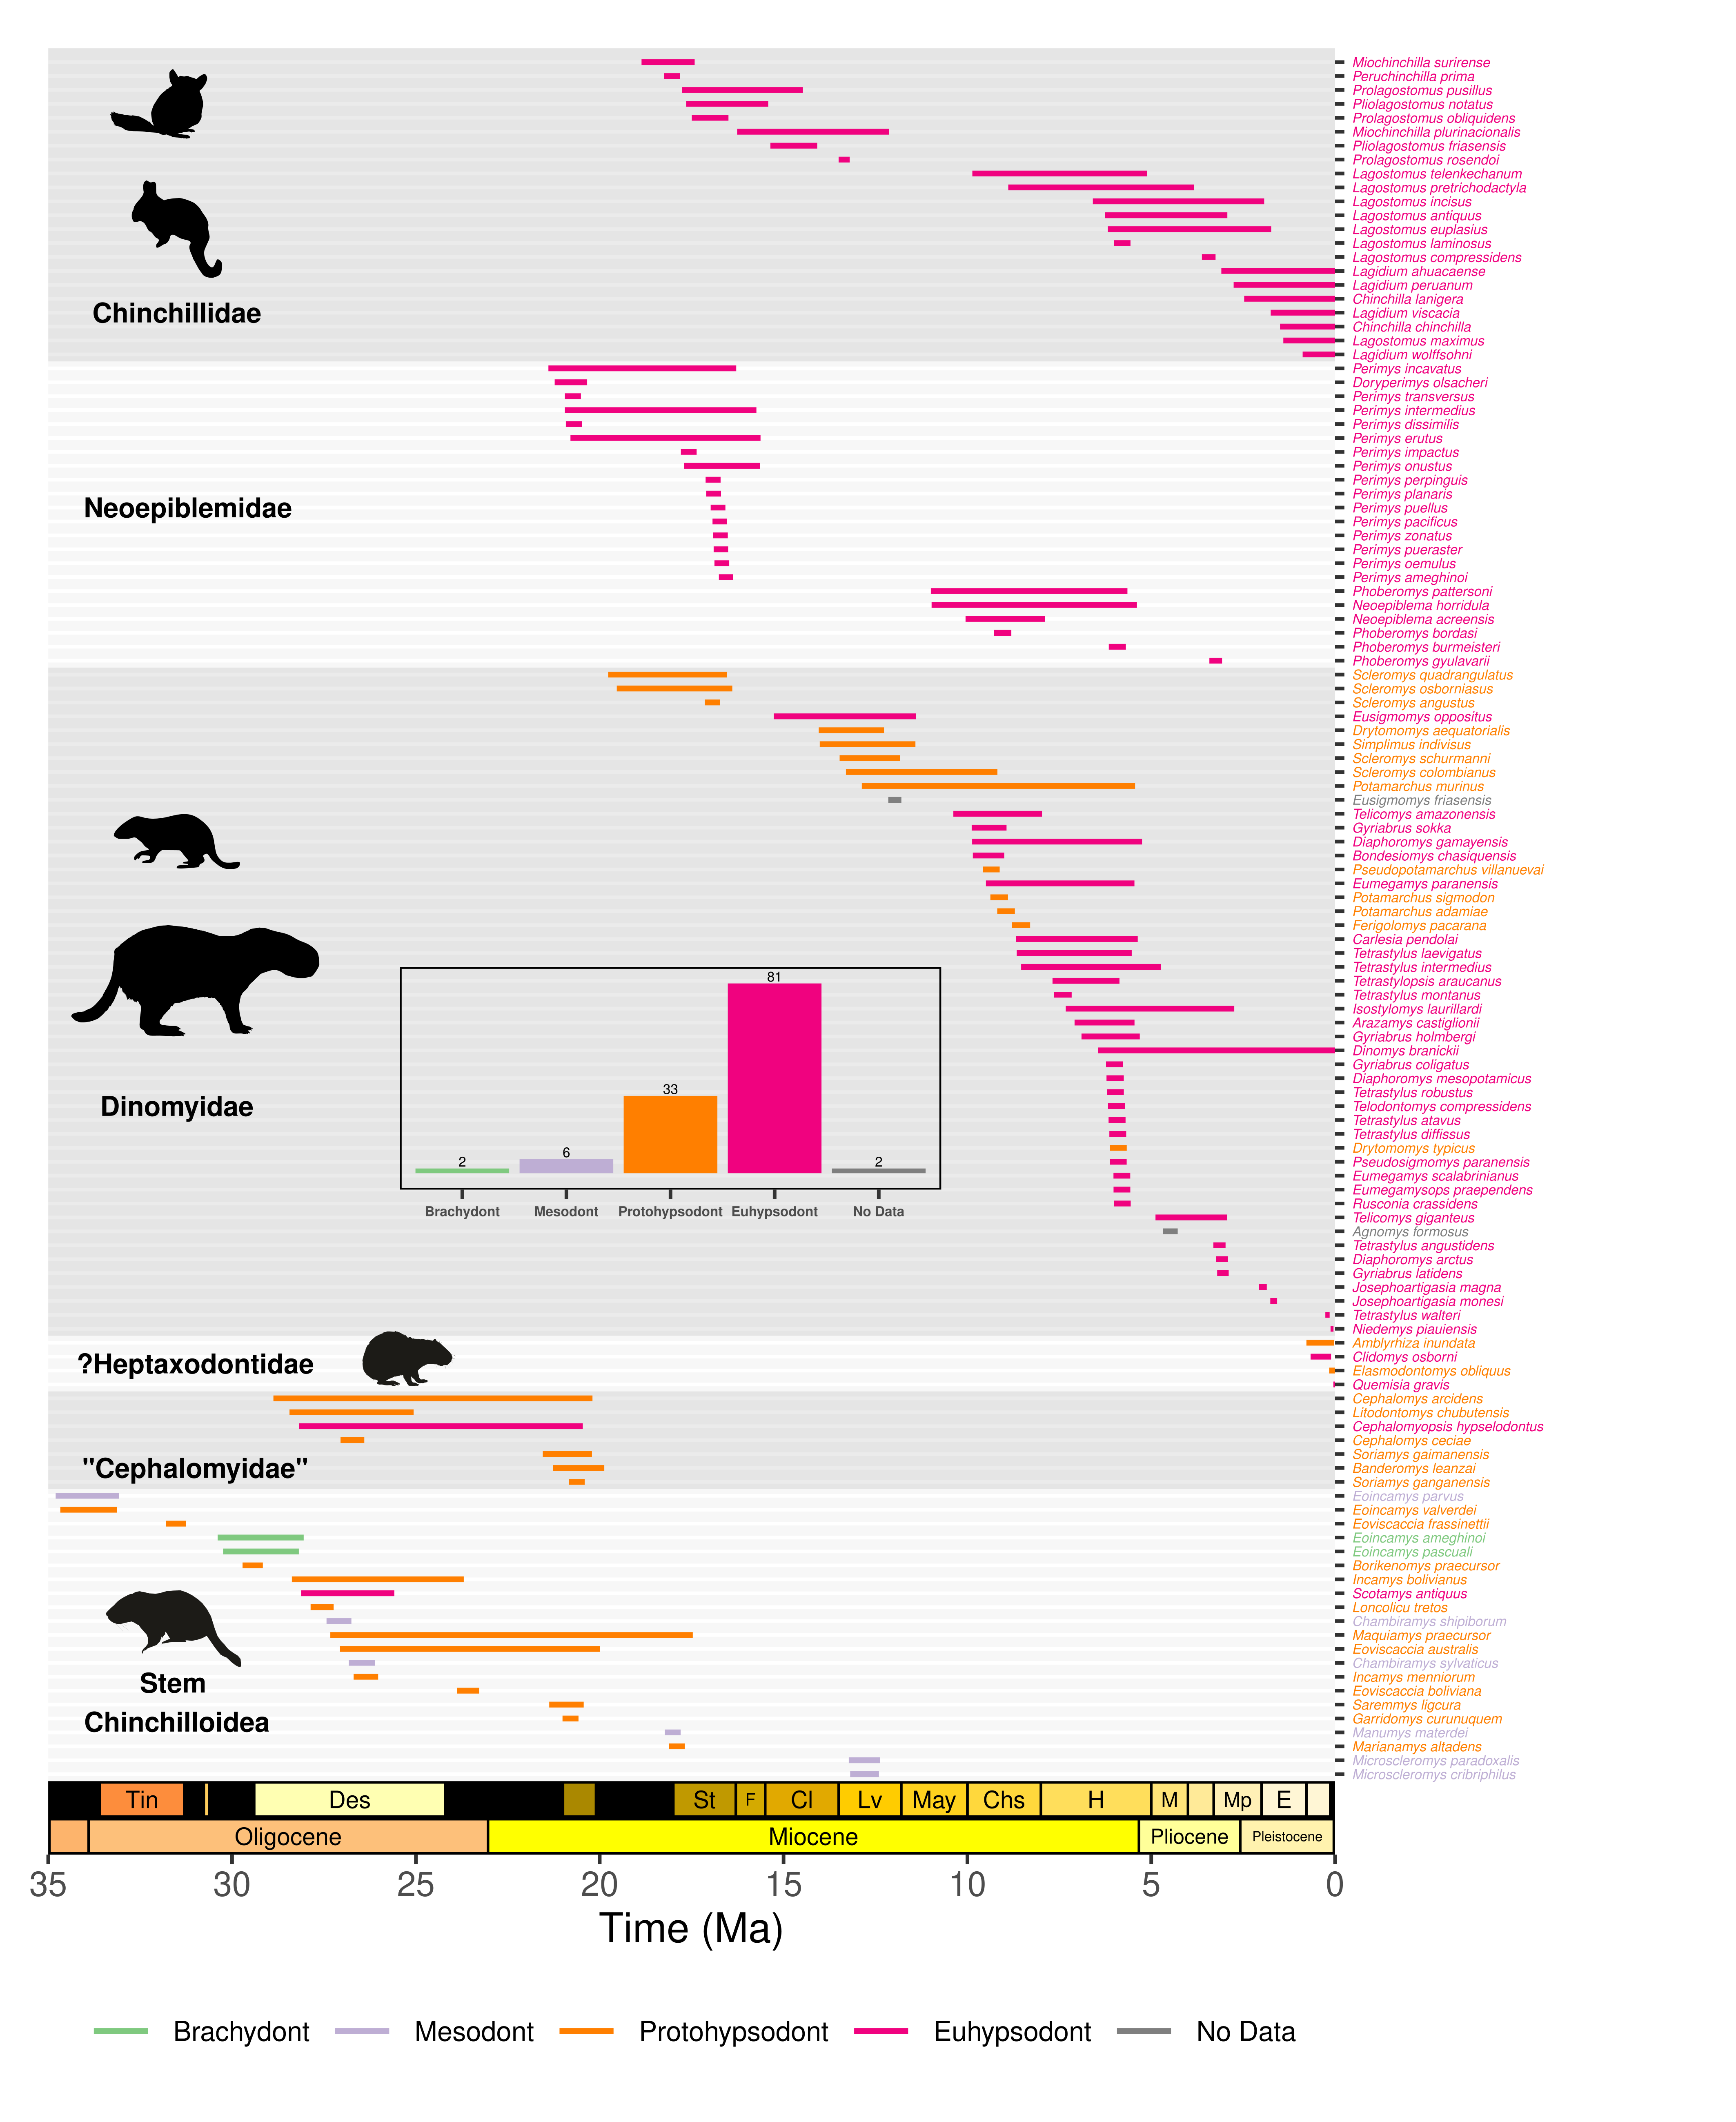
\includegraphics[width=14.17in,height=18cm]{../../Figures/Supp/Lifespans_hypso/Lifespans_HI_Chinchi.png}

}

\caption{\label{fig-LifespanHypso}Bayesian reconstruction of the
longevities of the 124 chinchilloid species considered in our dataset.
Each segment depicts the longevity of a given species, that is, the
interval between species' speciation and extinction times averaged
across PyRate runs that achieved convergence. Segments and taxonomic
names were coloured according to the crown height category to which
species were assigned. The histogram at the centre of the plot shows the
number of species within each crown height class. Depending on the
phylogenetic hypothesis considered Rasia et al.
(\citeproc{ref-rasia_comprehensive_2021}{2021}), taxa labelled a `Stem
Chinchilloidea' may either be considered as actual stem, or as
\emph{Familia incertae sedis}. The first four silhouettes (from top to
bottom) are from Phylopic (credits available in Table S3). The last two
silhouettes (\emph{Elasmodontomys obliquus} and \emph{Borikenomys
praecursor}) were designed by L.M. for a previous work
(\citeproc{ref-marivaux_early_2020}{Marivaux et al. 2020}).}

\end{suppfigure}%

\begin{suppfigure}[H]

\centering{

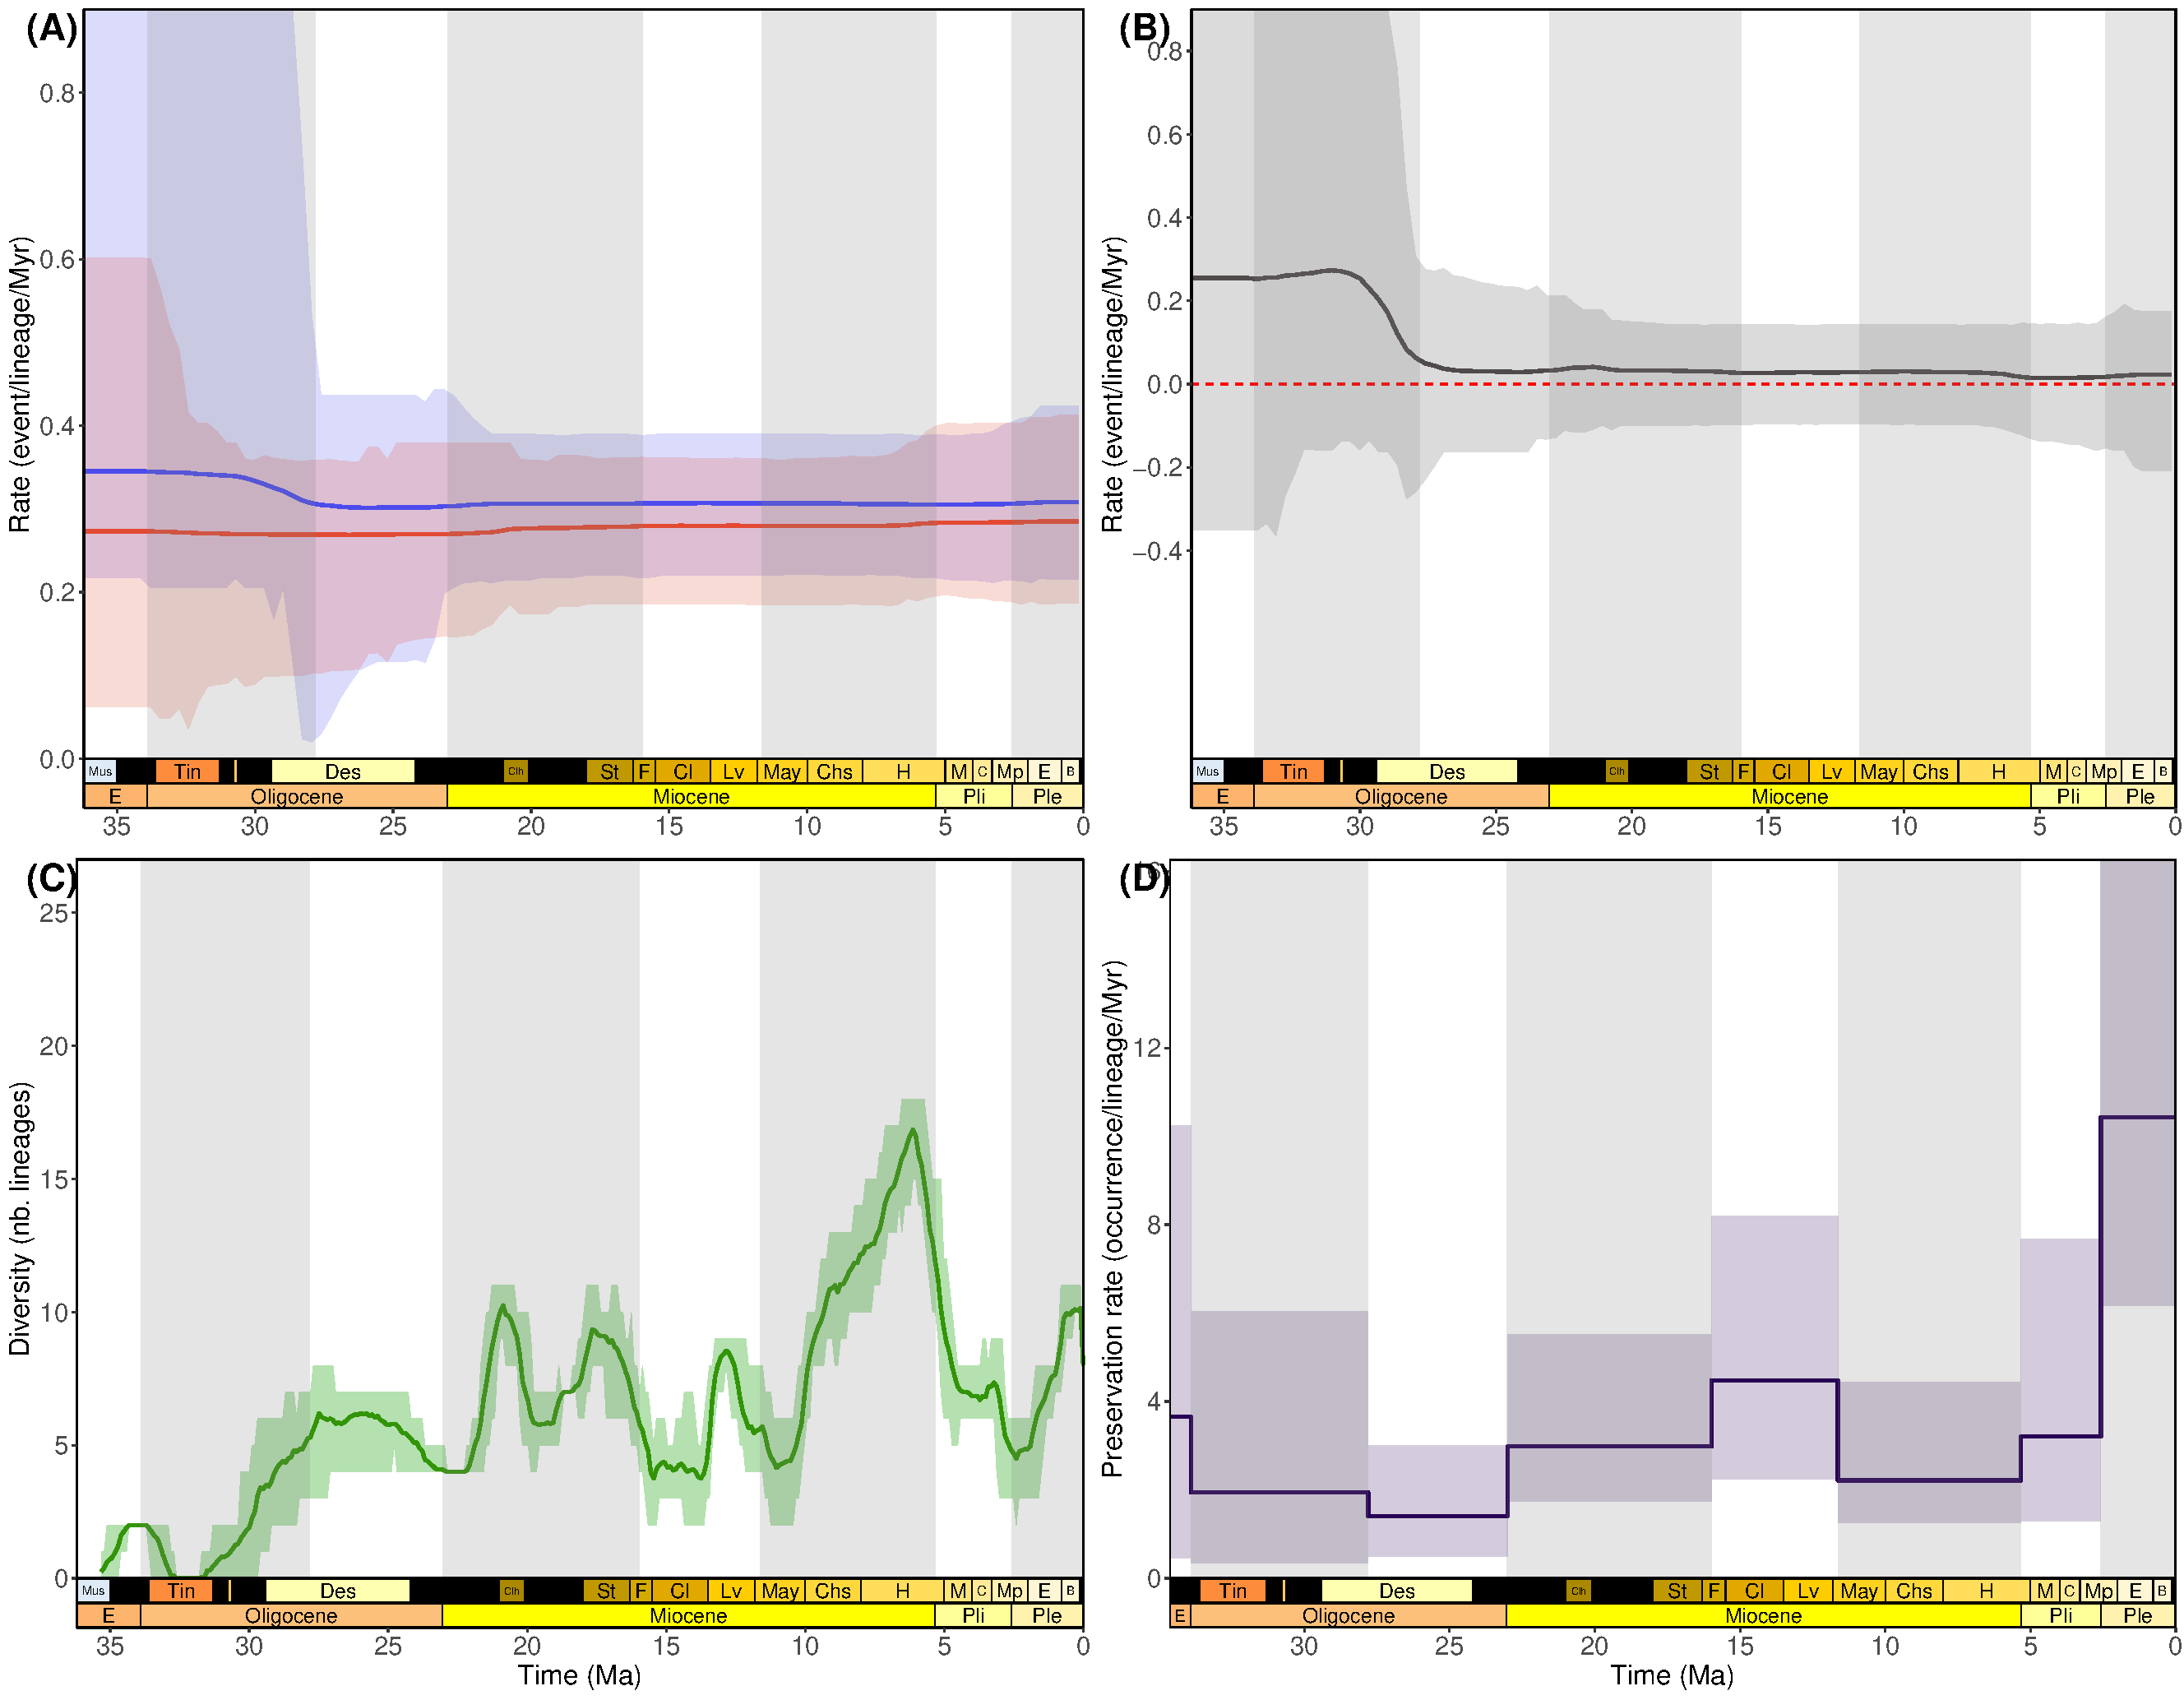
\includegraphics[width=\textwidth,height=10cm]{../../Figures/recap_figures_RJMCMC/New/Chinchilloidea_species_Singleton_Recap_figure.pdf}

}

\caption{\label{fig-RecapSingletonRTT}Joint estimation of origination
(blue) and extinction (red) rates (\textbf{A}), net diversification rate
(\textbf{B}), diversity through time (\textbf{C}) and preservation rates
(\textbf{D}) from our species-level chinchilloid database made my PyRate
(rjMCMC algorithm) after removing singletons.}

\end{suppfigure}%

\begin{suppfigure}[H]

\centering{

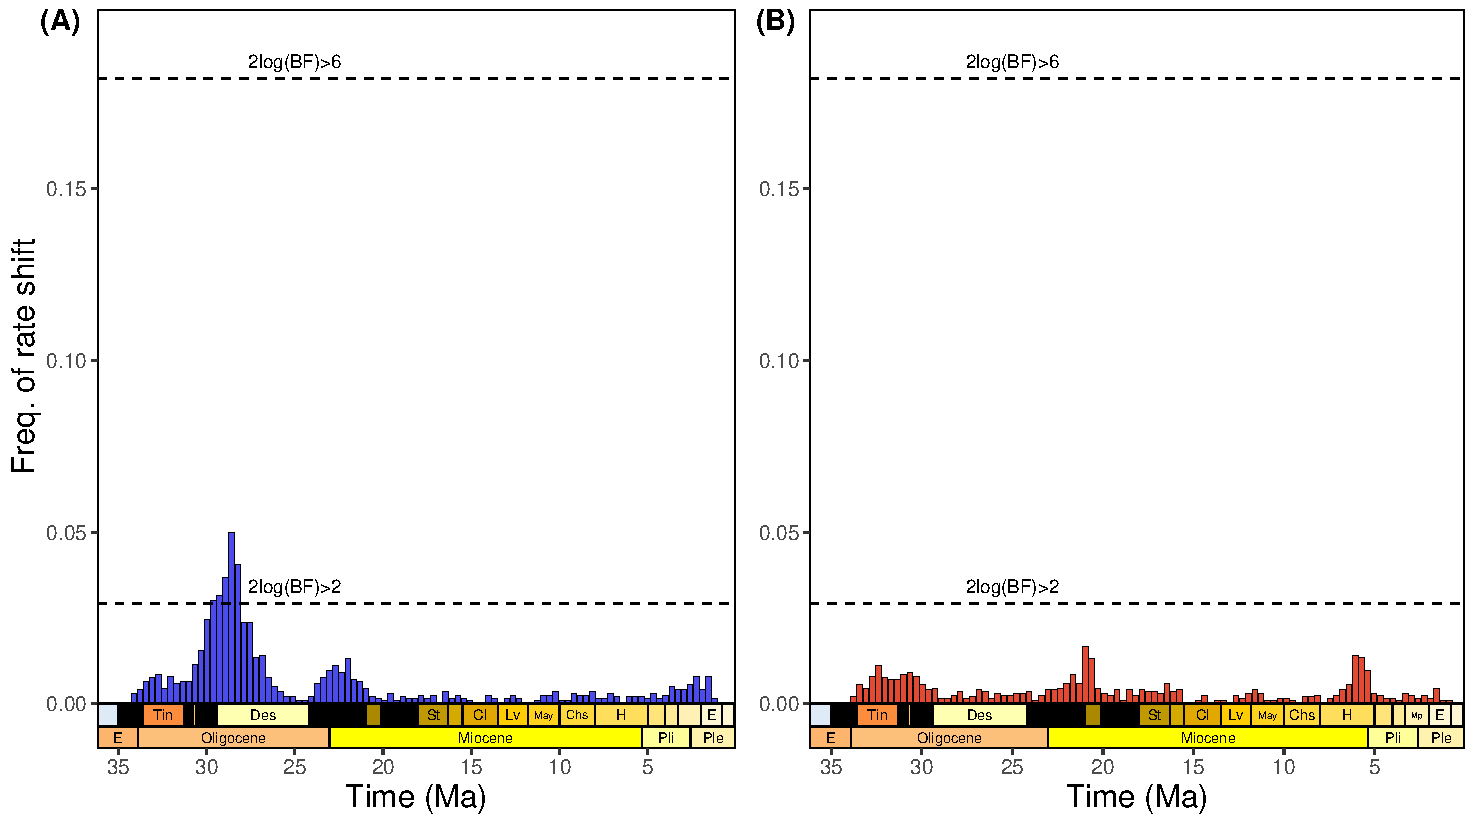
\includegraphics[width=\textwidth,height=8cm]{../../Figures/recap_figures_RJMCMC/New/Chinchilloidea_species_Singleton_frequency_of_rate_shift.pdf}

}

\caption{\label{fig-SingletonFRS}Frequency of origination (\textbf{A})
and extinction (\textbf{B}) rates estimated by the rjMCMC analysis of
our species-level database after removing singletons.}

\end{suppfigure}%

\begin{suppfigure}[H]

\centering{

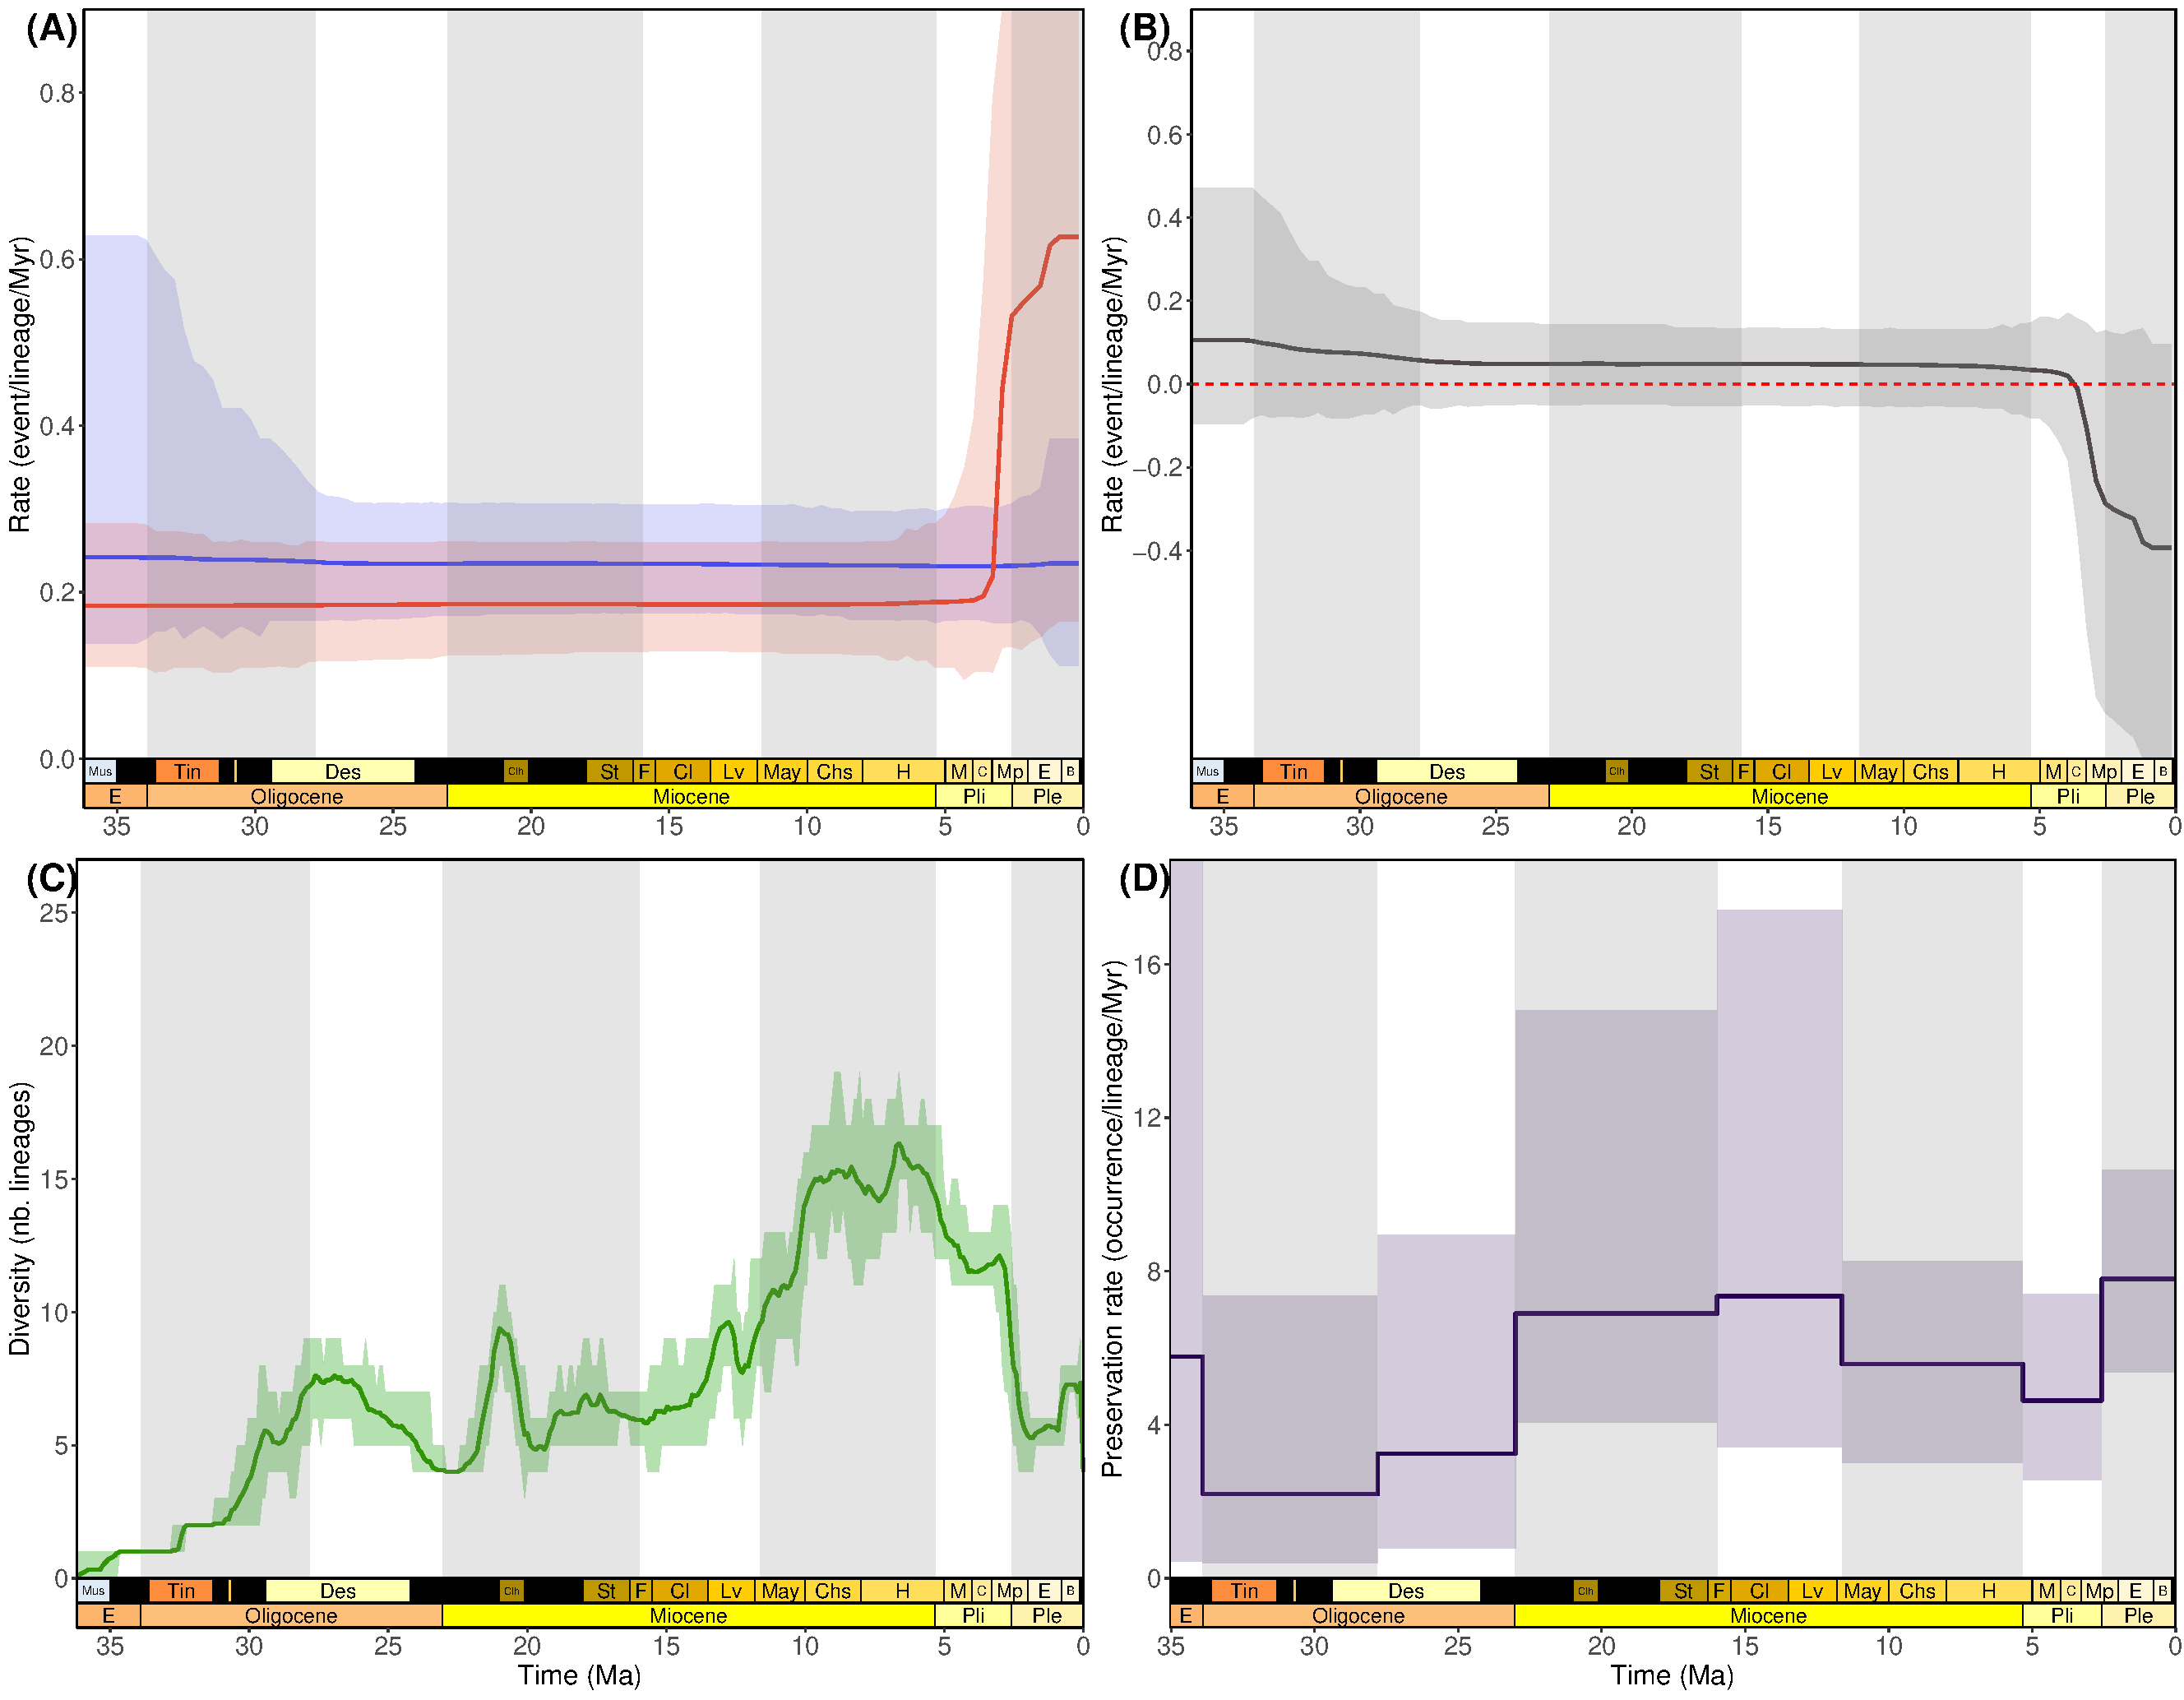
\includegraphics[width=\textwidth,height=10cm]{../../Figures/recap_figures_RJMCMC/New/Chinchilloidea_genus_Full_Recap_figure.pdf}

}

\caption{\label{fig-RecapGenRTT}Joint estimation of origination (blue)
and extinction (red) rates (\textbf{A}), net diversification rate
(\textbf{B}), diversity through time (\textbf{C}) and preservation rates
(\textbf{D}) from the genus-level chinchilloid database made my PyRate
(rjMCMC algorithm).}

\end{suppfigure}%

\begin{suppfigure}[H]

\centering{

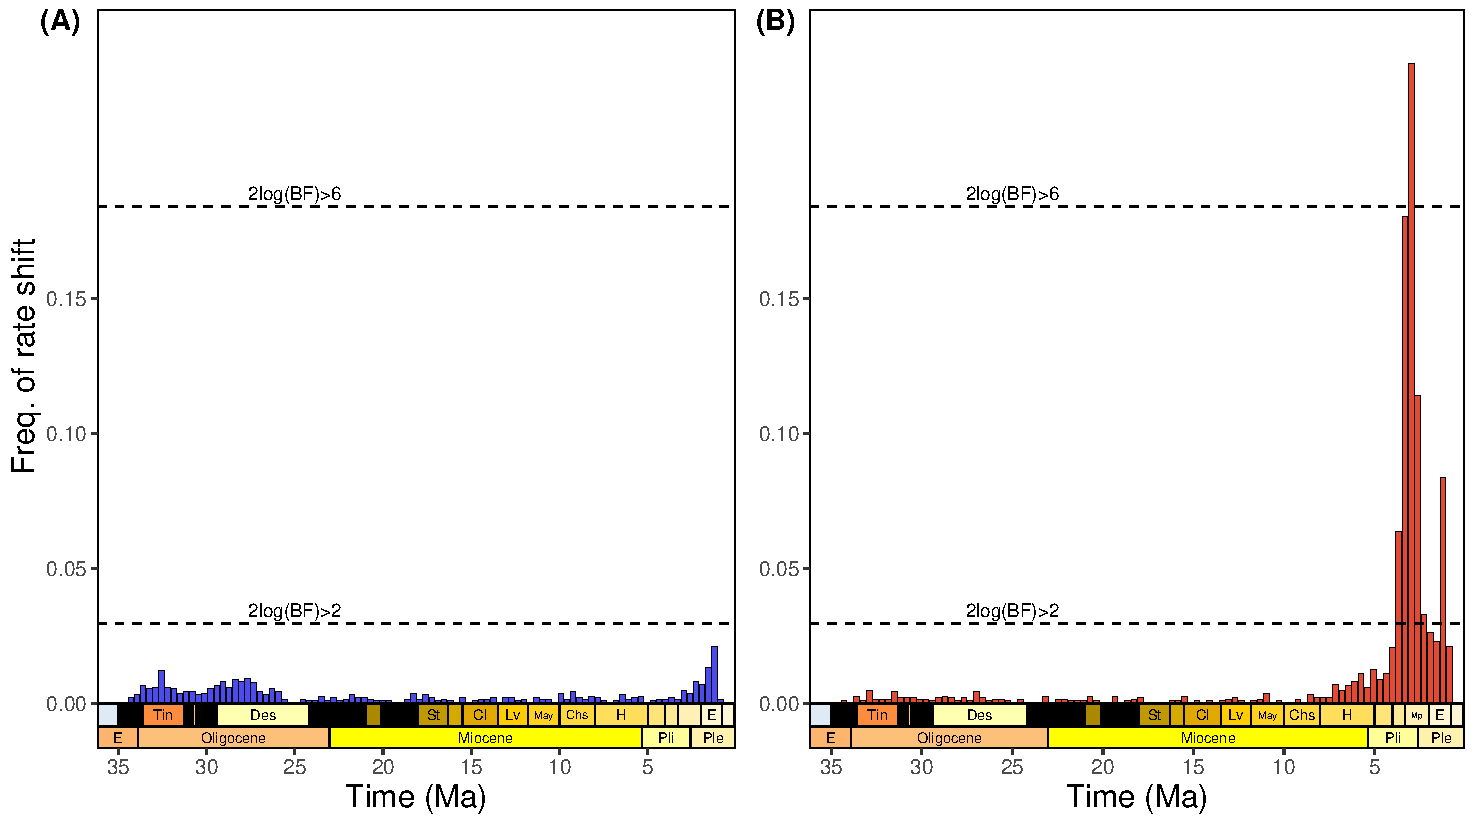
\includegraphics[width=\textwidth,height=8cm]{../../Figures/recap_figures_RJMCMC/New/Chinchilloidea_genus_Full_frequency_of_rate_shift.pdf}

}

\caption{\label{fig-FRSGen}Frequency of origination (\textbf{A}) and
extinction (\textbf{B}) rates estimated by the rjMCMC analysis of our
genus-level database.}

\end{suppfigure}%

\begin{suppfigure}[H]

\centering{

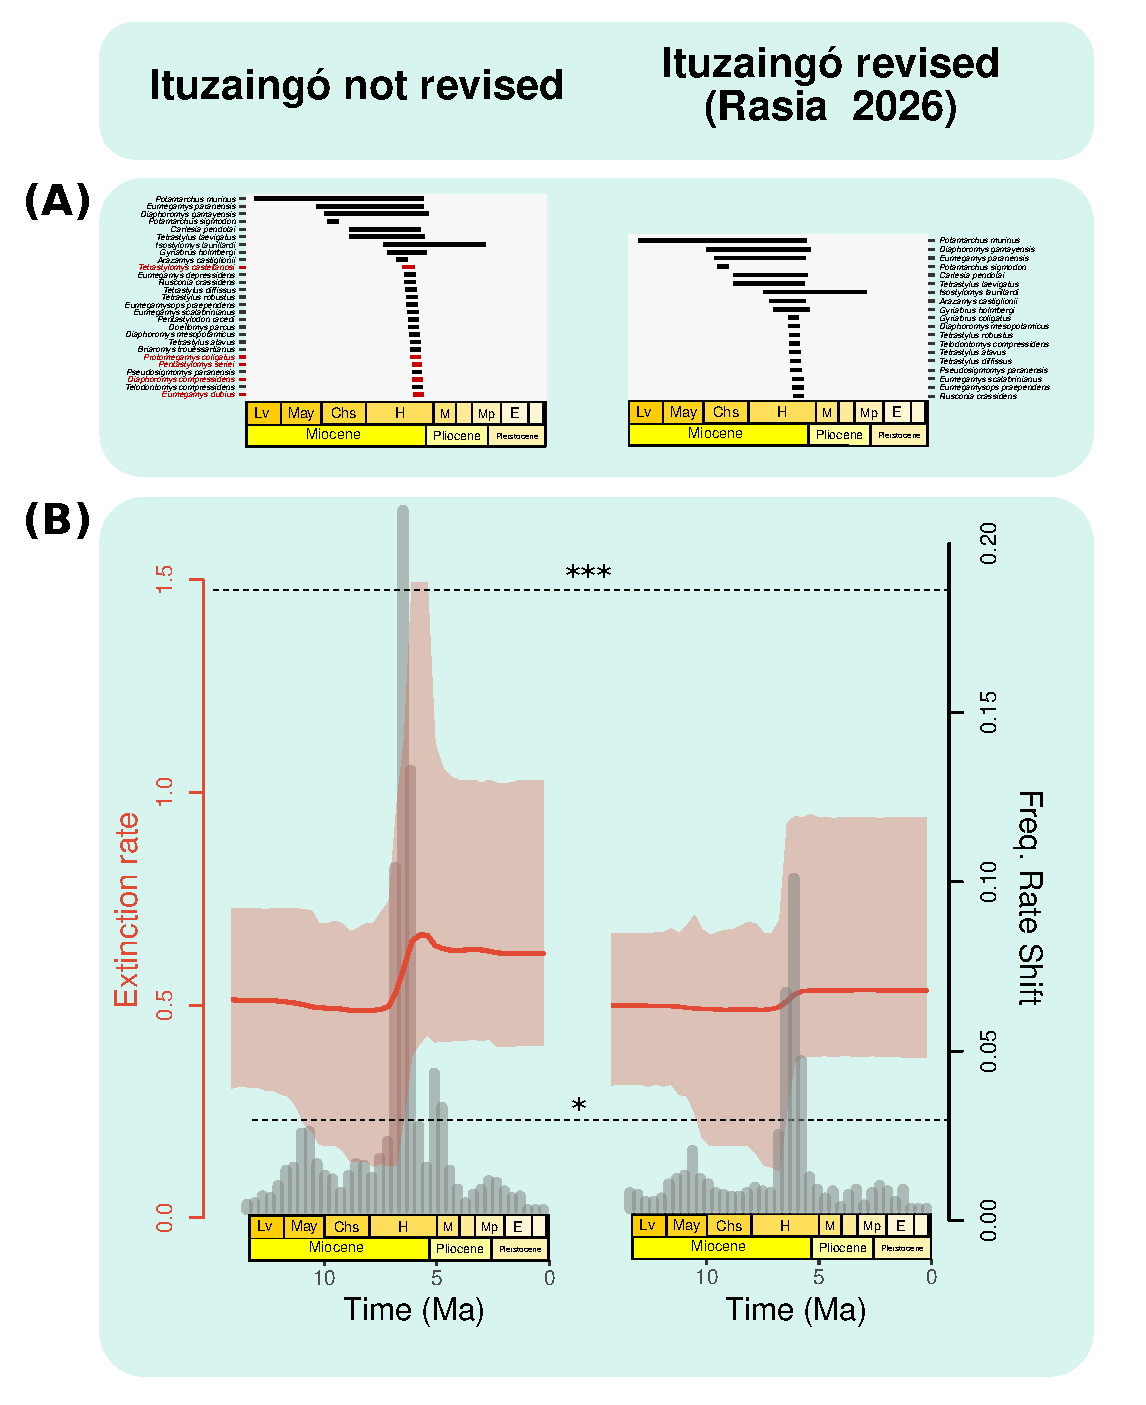
\includegraphics[width=\textwidth,height=19cm]{../../Figures/Supp/Effect_Rasia2026/rasia_effect.pdf}

}

\caption{\label{fig-RasiaEffect}Impact of accounting for the revision of
the dinomyid fauna of the Ituzaingó Formation (Entre Ríos Province,
Argentina) on the estimation of the temporal dynamics of chinchilloid
extinction rate (\citeproc{ref-rasia2026}{Rasia 2026}). (\textbf{A})
Lifespans of species making up the `Mesopotamiense' fauna (Ituzaingó
Fm.) before (\emph{left}) and after (\emph{right}) the taxonomic
revision. Removed taxa were coloured in red (five taxa lost).
(\textbf{B}) Chinchilloid extinction rates estimated from our temporal
occurrence database before (\emph{left}) and after (\emph{right})
incorporating the aforementioned revision. The histogram in background
shows the frequency of rate shift estimated by the rjMCMC model, that
is, for a given time frame (by default set to 1My), how likely it is to
consider that the reconstructed extinction rate experienced a shift. The
dashed lines labelled (*) and (***) respectively indicate significant
and strongly supported rate shift.}

\end{suppfigure}%

\begin{suppfigure}[H]

\centering{

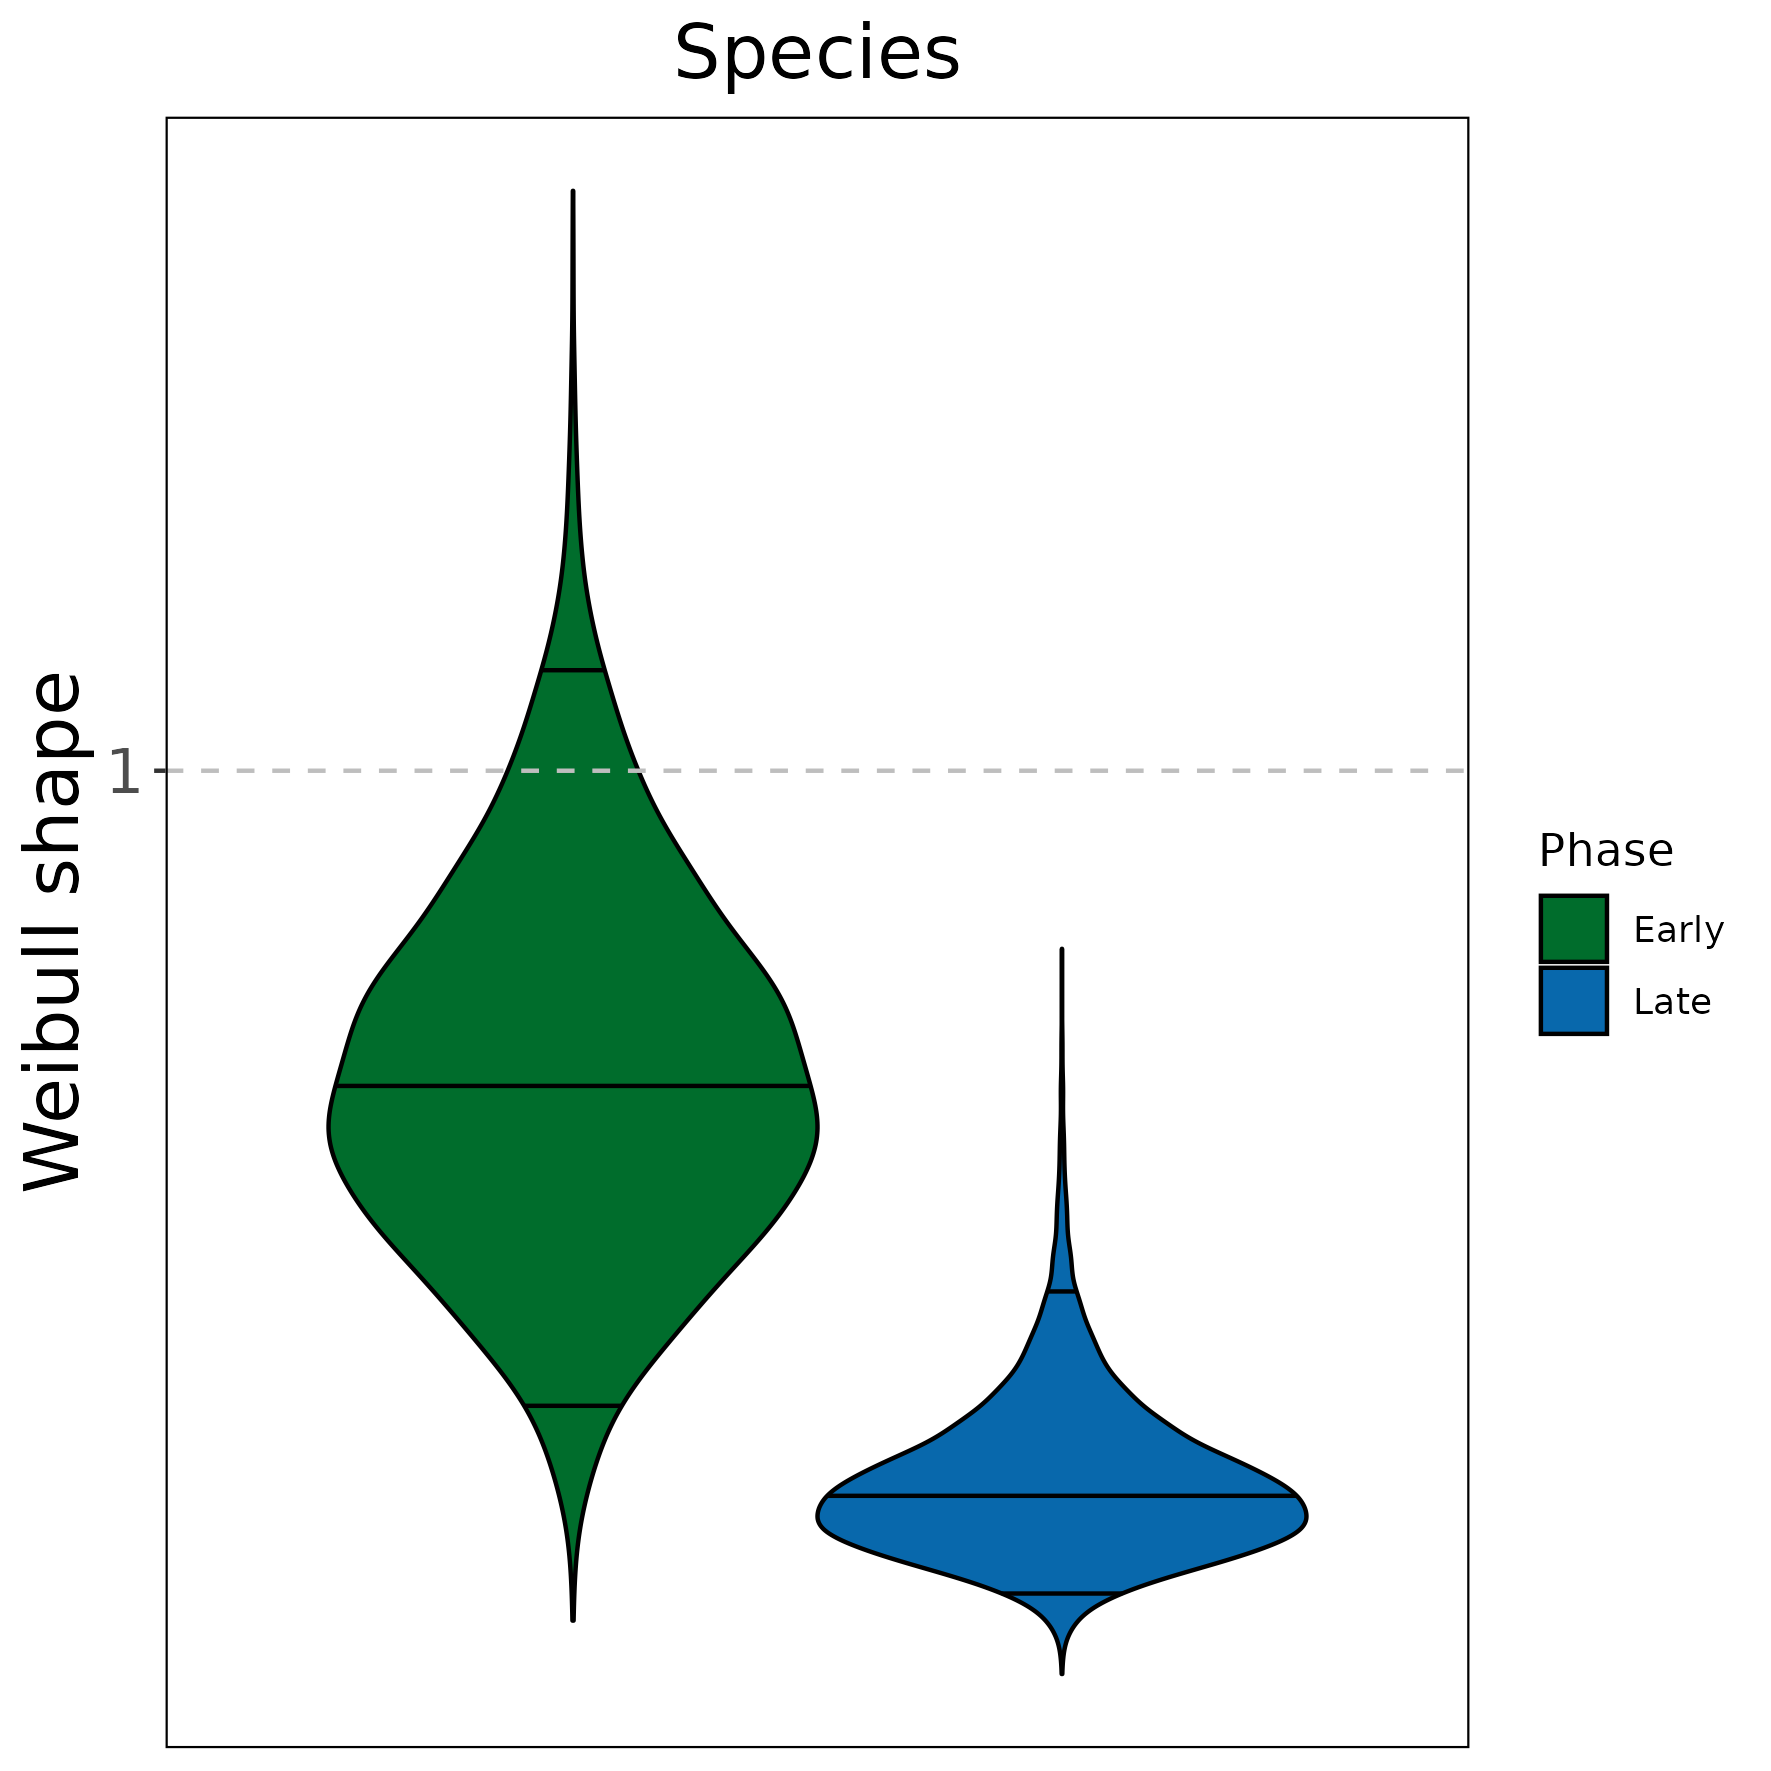
\includegraphics[width=15cm,height=7.5cm]{../../Figures/ADE/Weibull_shape_species.png}

}

\caption{\label{fig-violinADE}Posterior estimate of the shape parameter
of the Weibull distribution for the ADE analyses of the `Early'
(\textgreater{} 6 Ma) and `Late' (\textless{} 6 Ma) occurrence datasets,
each with constant extinction rate (Figure~S\ref{fig-FreqRateShift}).
2.5\%, 50\% and 97.5\% quantiles are indicated in the distribution of
each parameter by black horizontal lines, respectively from bottom to
top.}

\end{suppfigure}%

\hfill\break
\hfill\break

\begin{suppfigure}[H]

\centering{

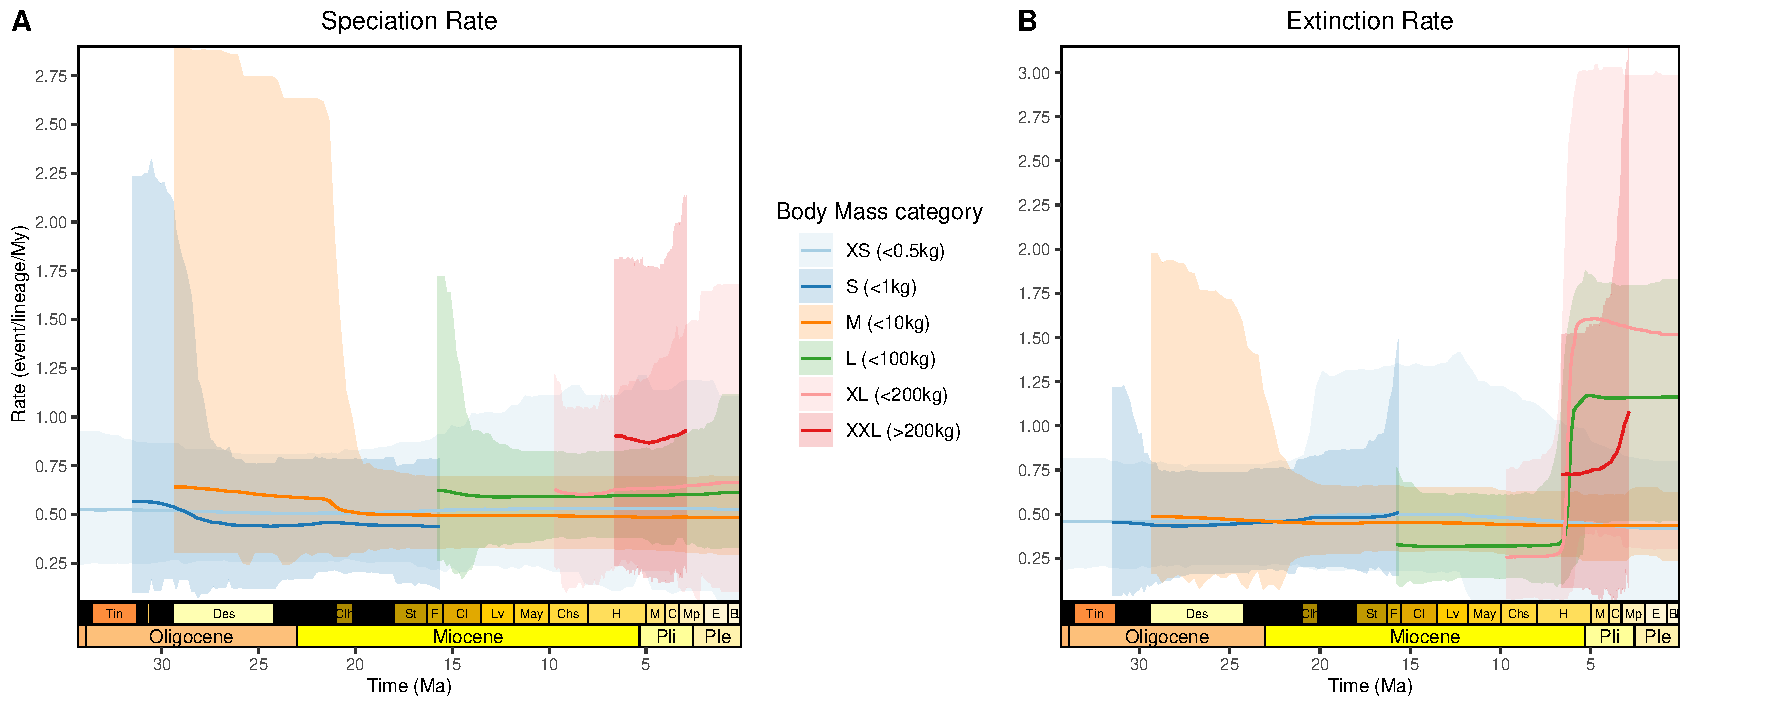
\includegraphics{../../Figures/Supp/RTT_per_BM/RTT_plot_per_BM.pdf}

}

\caption{\label{fig-RTTperBM}Speciation (\textbf{A}) and extinction
(\textbf{B}) rates through time per body mass class as inferred by the
rjMCMC model.}

\end{suppfigure}%

\begin{suppfigure}[H]

\centering{

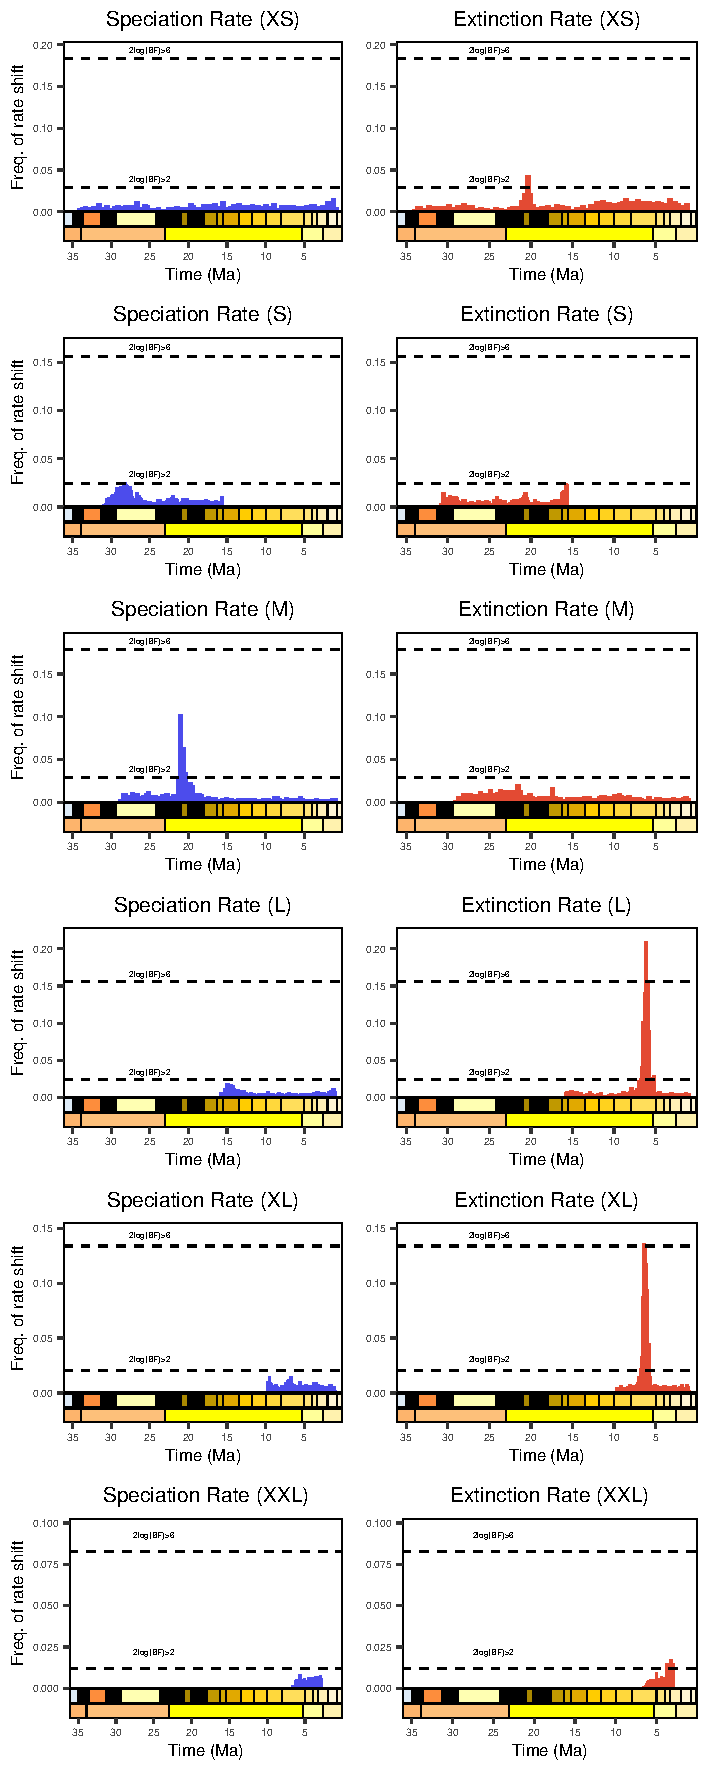
\includegraphics{../../Figures/Supp/RTT_per_BM/freq_rate_shift_per_BM.pdf}

}

\caption{\label{fig-FreqRateShiftBM}Frequency of speciation and
extinction rate shifts per body size class as estimated by the analysis
of our species-level chinchilloid occurrence dataset with the rjMCMC
model. Dashed horizontal lines indicate 2 * log(Bayes factor) of 2 and
6, respectively suggesting significant and strongly-supported rate
shifts.}

\end{suppfigure}%

\begin{suppfigure}[H]

\centering{

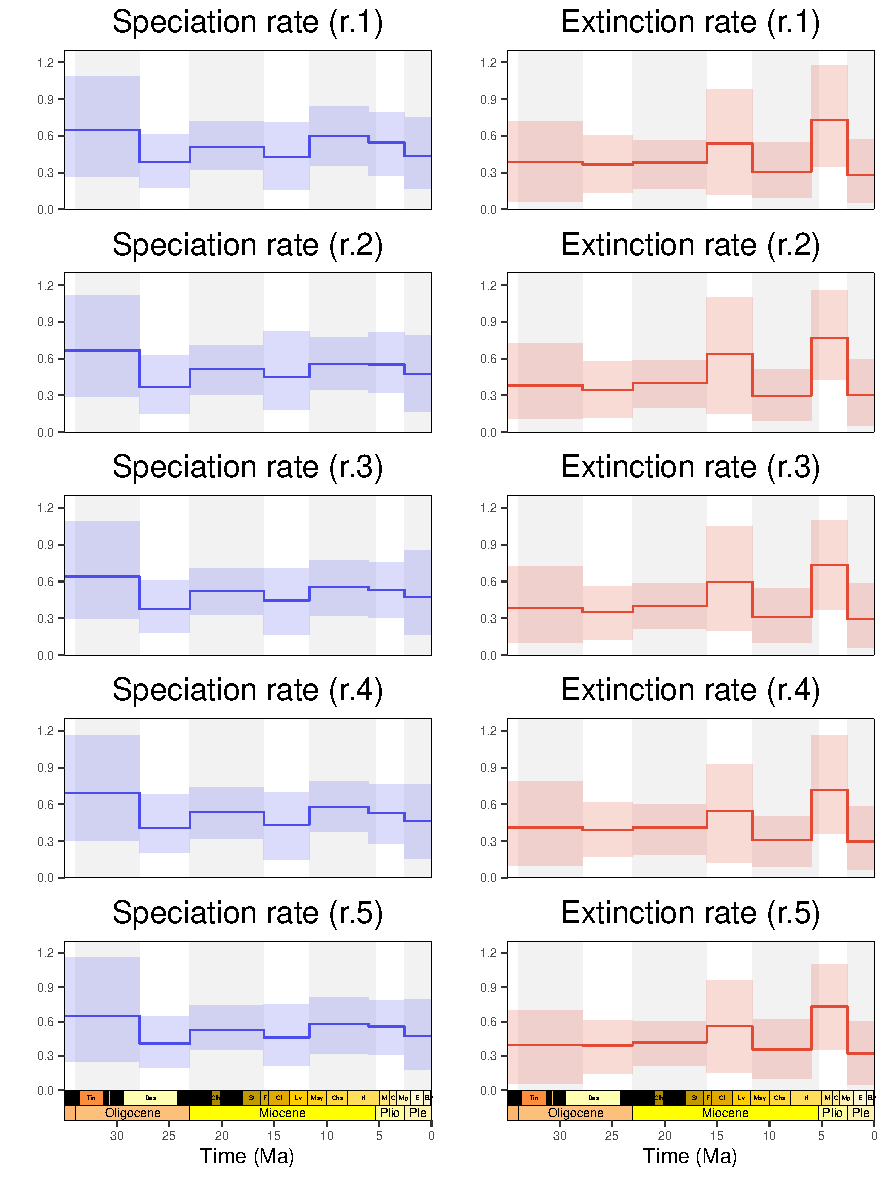
\includegraphics{../../Figures/Supp/RTT_imputation/RTT_imput_full_NoCar15.pdf}

}

\caption{\label{fig-RTT_BDNN_NoCar15}Marginal chinchilloid speciation
(blue) and extinction (red) rates through time as estimated by our BDNN
analyses of the datasets with random trait (\emph{i}.\emph{e}., body
mass and/or hypsodonty index) imputation for taxa with missing trait
reconstruction (\(n=11\)). Caribbean taxa were excluded. Full lines show
median rate estimates and ribbons their associated 95\% Highest
Posterior Density (HPD) interval, assessed acrossed the 10 independent
BDNN runs randomising fossil ages under a uniform law made for each
trait imputation. This panel only depicts the rates through time from
replicate 1 to 5.}

\end{suppfigure}%

\begin{suppfigure}[H]

\centering{

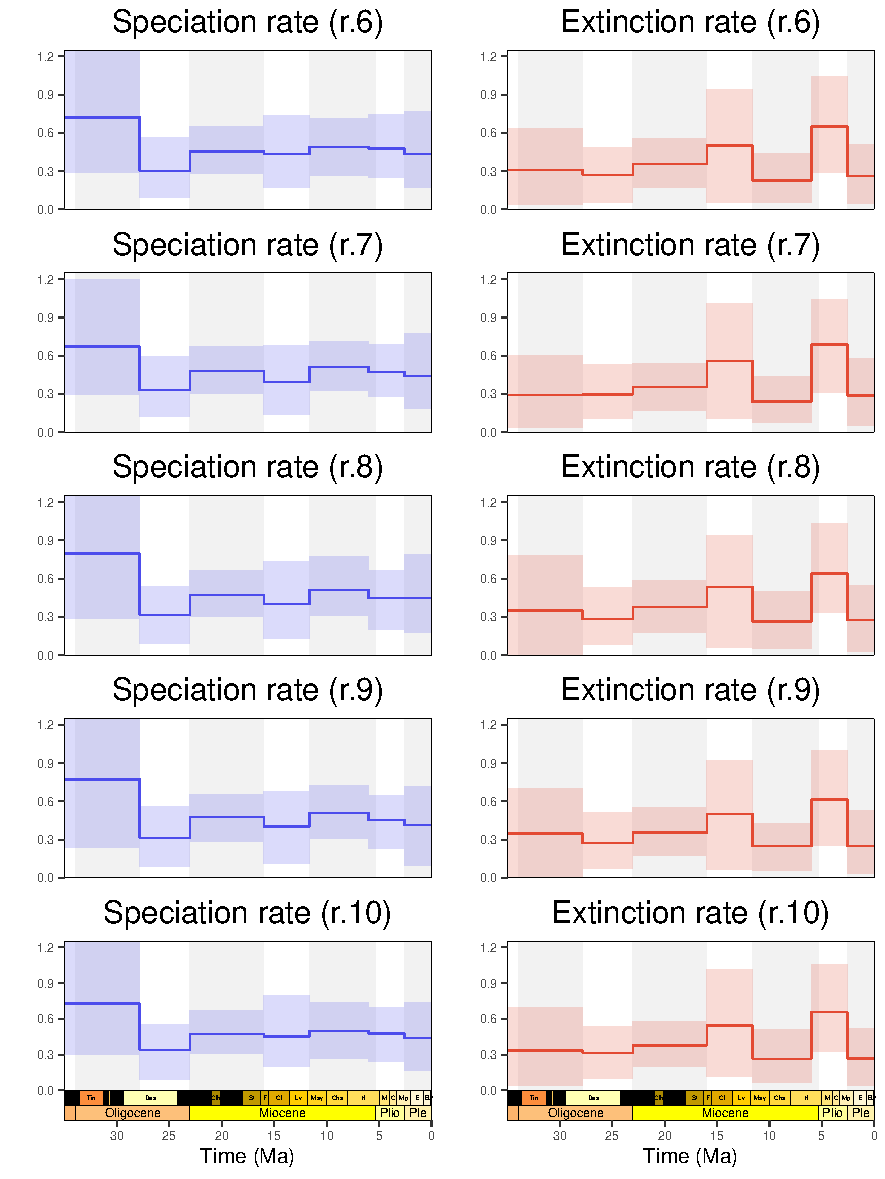
\includegraphics{../../Figures/Supp/RTT_imputation/RTT_imput_full_NoCar610.pdf}

}

\caption{\label{fig-RTT_BDNN_NoCar610}Marginal chinchilloid speciation
(blue) and extinction (red) rates through time as estimated by our BDNN
analyses of the datasets with random trait (\emph{i}.\emph{e}., body
mass and/or hypsodonty index) imputation for taxa with missing trait
reconstruction (\(n=11\)). Caribbean taxa were excluded. Full lines show
median rate estimates and ribbons their associated 95\% Highest
Posterior Density (HPD) interval, assessed acrossed the 10 independent
BDNN runs randomising fossil ages under a uniform law made for each
trait imputation. This panel only depicts the rates through time from
replicate 1 to 5.}

\end{suppfigure}%

\begin{suppfigure}[H]

\centering{

\includegraphics[width=20cm,height=7.5cm]{../../Results/DeepDive/species_extant_extended/species_extant_extended_models/simulation_species_extant_extended_ET_20260224_lstm128_64_32_d64_32_conditional/history_plotsimulation_species_extant_extended_ET_20260224_lstm128_64_32_d64_32_conditional.pdf}

}

\caption{\label{fig-ddHistPlotL2D2}Training and validation loss across
training epochs for a DeepDive network comprising two LSTM units (64 and
32 nodes) connected to two dense layers (64 and 32 nodes) before the
output layer. The red vertical line indicates the ``early stopping
point'', \emph{i}.\emph{e}., when the validation loss starts increasing,
indicative of overfitting. It determines the optimal value of number of
iterations, at which we derive the training and validation loss values
depicted between parenthesis.}

\end{suppfigure}%

\begin{suppfigure}[H]

\centering{

\includegraphics[width=20cm,height=7.5cm]{../../Results/DeepDive/species_extant_extended/species_extant_extended_models/simulation_species_extant_extended_ET_20260224_lstm64_32_d64_32_conditional/history_plotsimulation_species_extant_extended_ET_20260224_lstm64_32_d64_32_conditional.pdf}

}

\caption{\label{fig-ddHistPlotL3D2}Training and validation loss across
training epochs for a DeepDive network comprising three LSTM units (128,
64 and 32 nodes) connected to two dense layers (64 and 32 nodes) before
the output layer. The red vertical line indicates the ``early stopping
point'', \emph{i}.\emph{e}., when the validation loss starts increasing,
indicative of overfitting. It determines the optimal value of number of
iterations, at which we derive the training and validation loss values
depicted between parenthesis.}

\end{suppfigure}%

\begin{suppfigure}[H]

\centering{

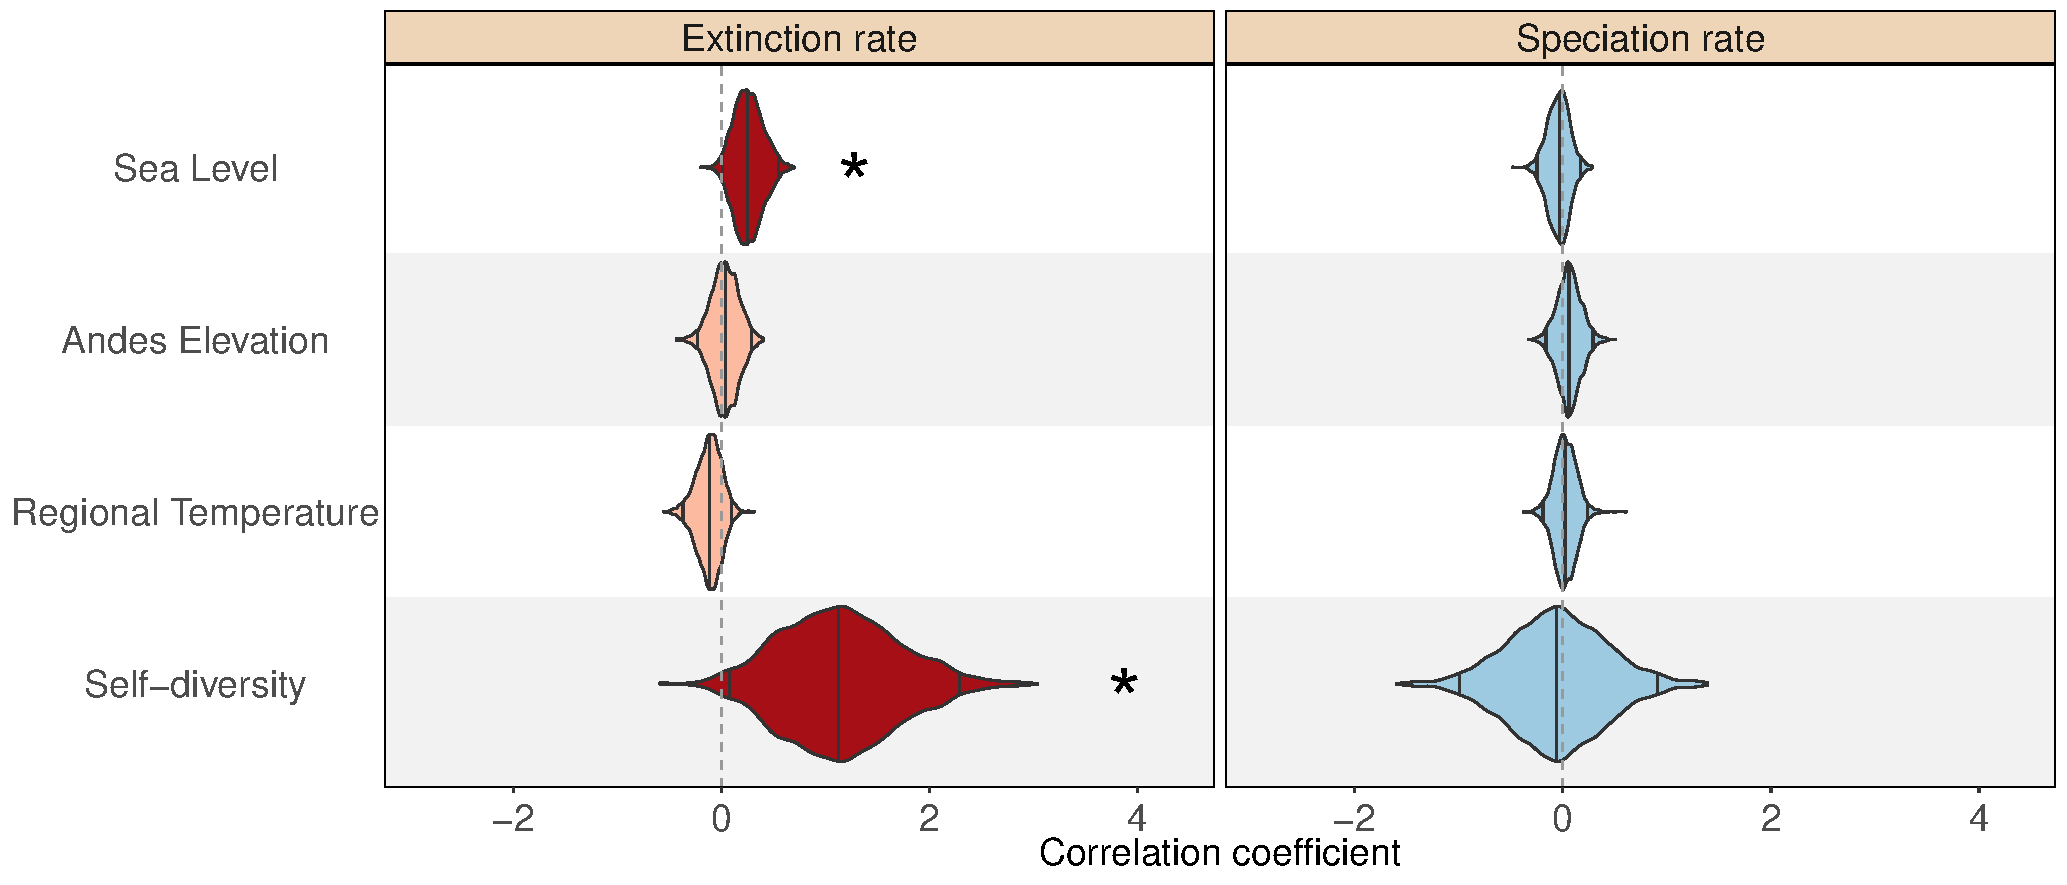
\includegraphics{../../Figures/Main/Drivers/MBD_species_complete_scaled_hsp0.pdf}

}

\caption{\label{fig-MBDcorrelations}Bayesian estimation of correlation
coefficients of extinction (\emph{left}) and speciation (\emph{right})
rates with a selected set of environmental variable carried out by the
MBD model (\emph{see Methods in the main text}). A gamma prior was set
to correlation parameters. Light colours (respectively blue for
speciation and red for extinction) indicate non-significant
correlations, and plain colours indicate significant correlations. A
correlation was considered to be significant if 0 was not included in
the parameter 95\% HPD interval.}

\end{suppfigure}%

\begin{suppfigure}[H]

\centering{

\includegraphics[width=\textwidth,height=10cm]{../../Results/comparing_with_Carrillo/persistence_violin.pdf}

}

\caption{\label{fig-Comprative_Persistence}Comparative persistence
(\emph{i}.\emph{e}., FAD minus LAD) of the 84 taxa in common between our
database (in blue) and Carrillo et al.
(\citeproc{ref-carrillo2026}{2026}). Mean persistences between the two
studies were compared with a paired Wilcoxon test.}

\end{suppfigure}%

\begin{suppfigure}[H]

\centering{

\includegraphics[width=20cm,height=25cm]{../../Results/comparing_with_Carrillo/comparative_LAD_FAD.pdf}

}

\caption{\label{fig-Comparative_LADFAD}Persistence in the fossil record
of the 84 species shared between our database (in blue) and Carrillo et
al. (\citeproc{ref-carrillo2026}{2026}) (in red). Persistence is
assessed as the interval between the First and Last Appearance Data
(resp. FAD and LAD) of each taxon.}

\end{suppfigure}%

\begin{suppfigure}[H]

\centering{

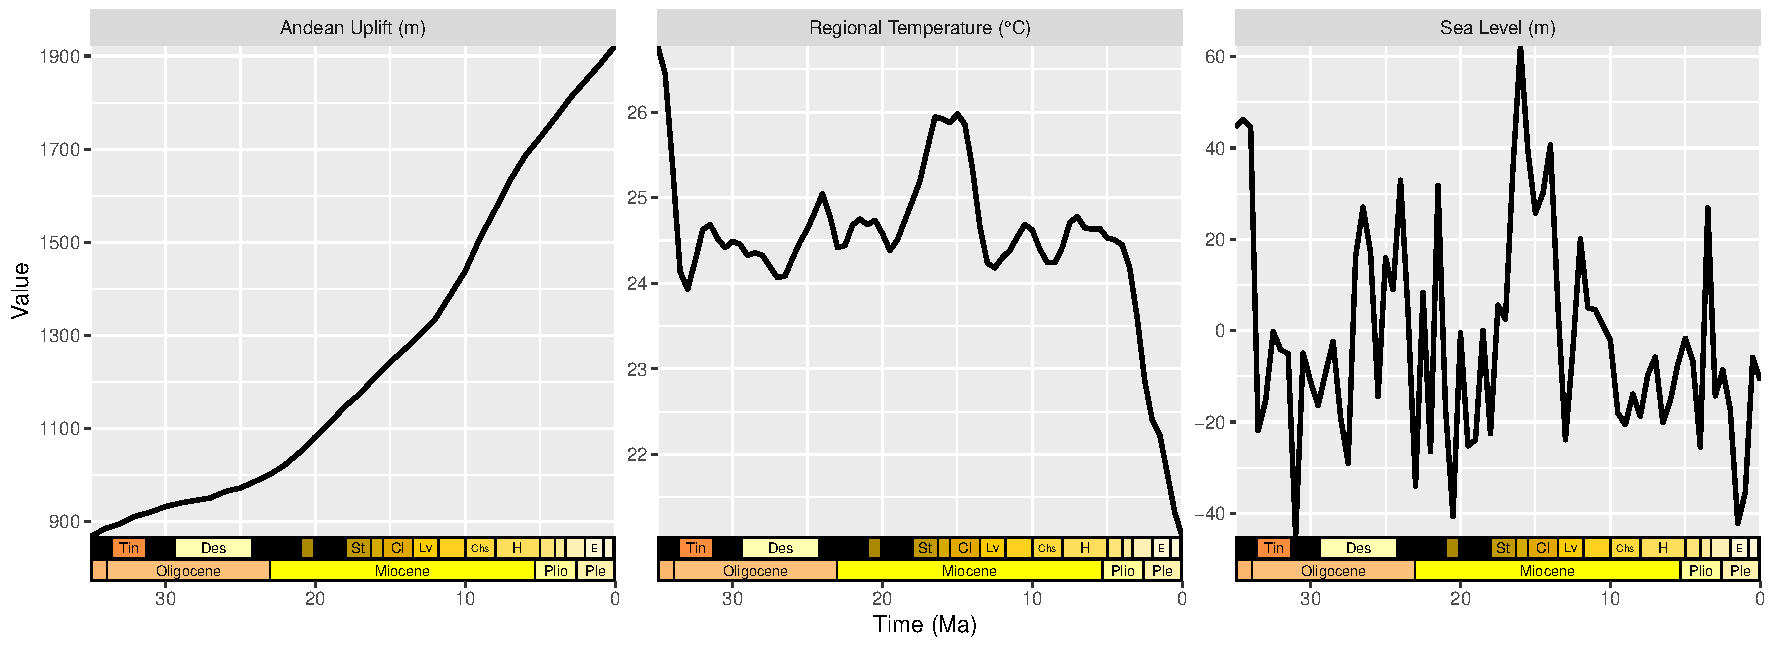
\includegraphics[width=16cm,height=\textheight]{../../Figures/Supp/Abiotic_correlates.pdf}

}

\caption{\label{fig-EnvCorrelates}Abiotic variables used in the
environment-dependent diversification analyses carried out over this
study. These have been temporally scaled to the same resolution
(500ky-step). Andean uplift was from Boschman
(\citeproc{ref-boschman2021}{2021}), South American regional temperature
was from Tardif et al. (\citeproc{ref-tardif2025}{2025}) and sea-level
changes were from Miller et al. (\citeproc{ref-miller2020}{2020}).}

\end{suppfigure}%

\begin{suppfigure}[H]

\centering{

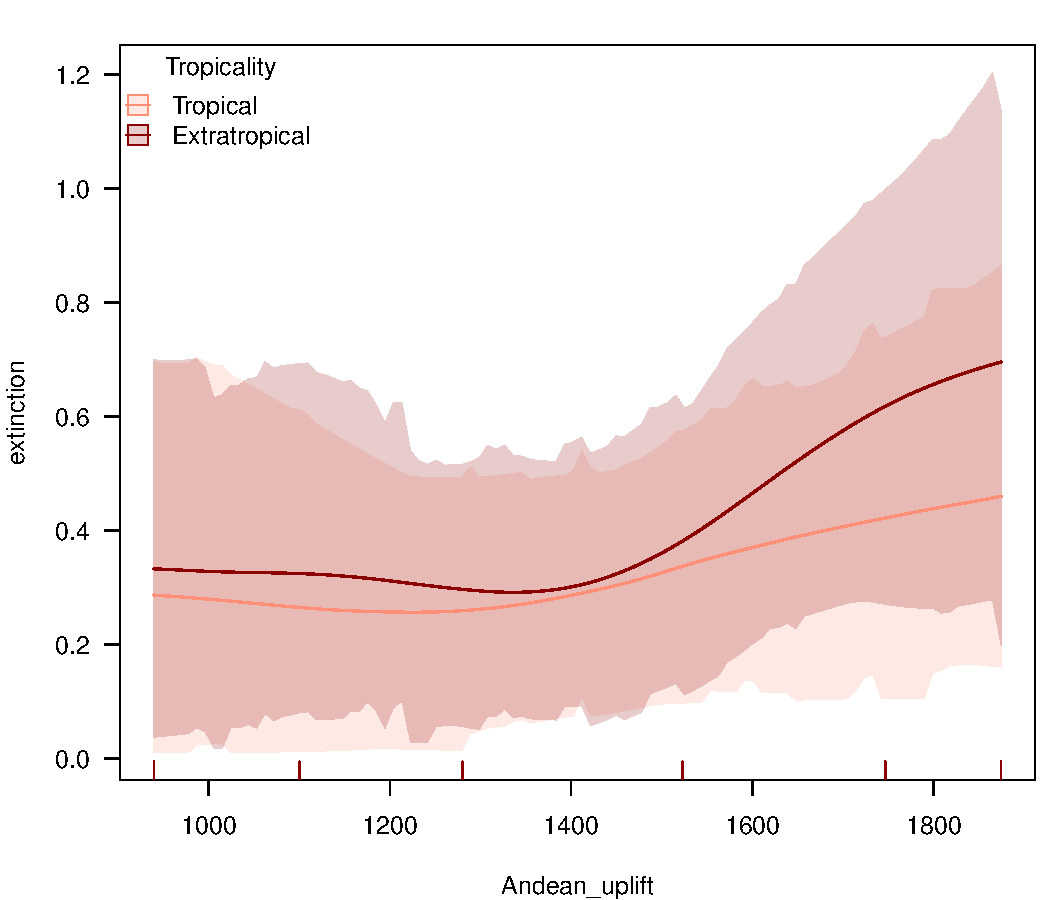
\includegraphics[width=13cm,height=\textheight]{../../Figures/Supp/Drivers_interaction/Upl_Tropicality.pdf}

}

\caption{\label{fig-UplTrop}Interaction between latitude and Andean
uplift in shaping chinchilloid extinction rate variations across
lineages, \emph{i}.\emph{e}., how the relationship between the Andean
uplift and extinction rate changes between tropical and extratropical
species. Results were arbitrarily taken from the third imputation
replicate of our BDNN analysis.}

\end{suppfigure}%

\begin{suppfigure}[H]

\centering{

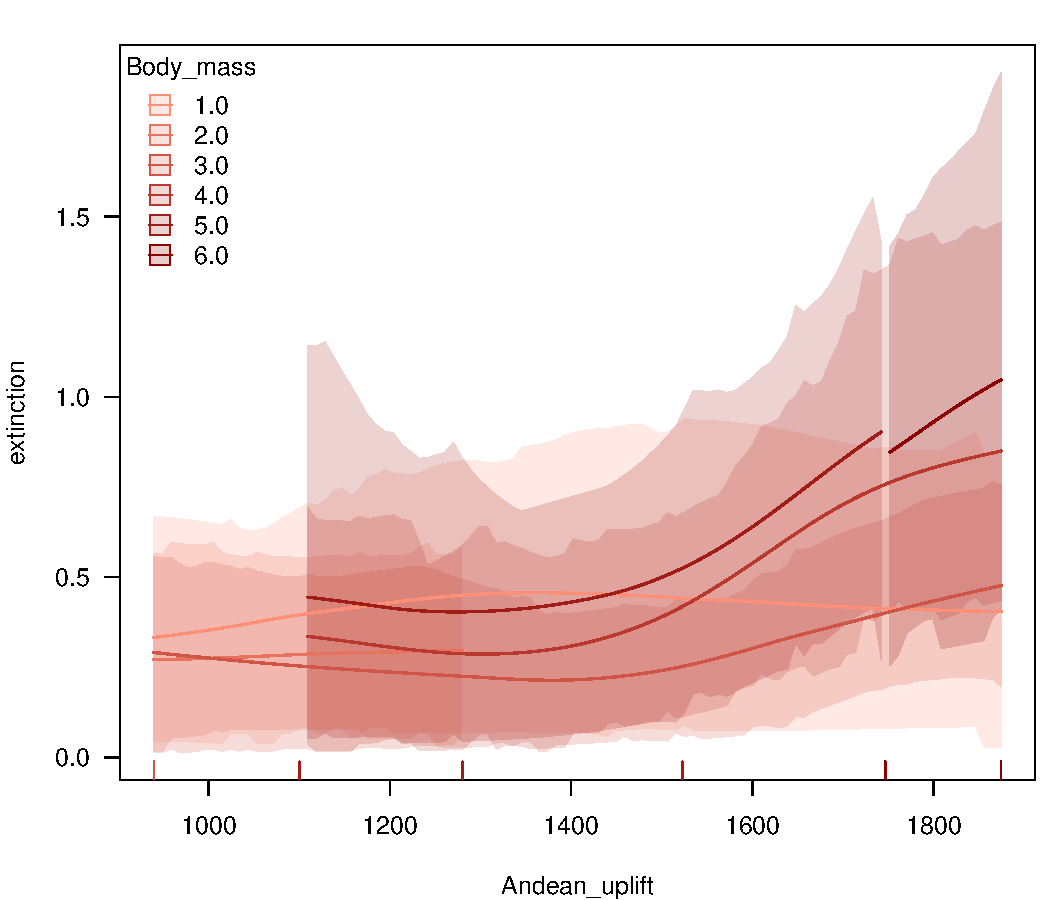
\includegraphics[width=13cm,height=\textheight]{../../Figures/Supp/Drivers_interaction/Upl_BM.pdf}

}

\caption{\label{fig-UplBM}Interaction between body mass and Andean
uplift in shaping chinchilloid extinction rate variations across
lineages, \emph{i}.\emph{e}., how the relationship between the Andean
uplift and extinction rate changes between body mass categories. Body
mass categories are numbered from 1 to 6 by increasing order
(\emph{i}.\emph{e}., from XS to XXL). Results were arbitrarily taken
from the third imputation replicate of our BDNN analysis.}

\end{suppfigure}%

\begin{suppfigure}[H]

\centering{

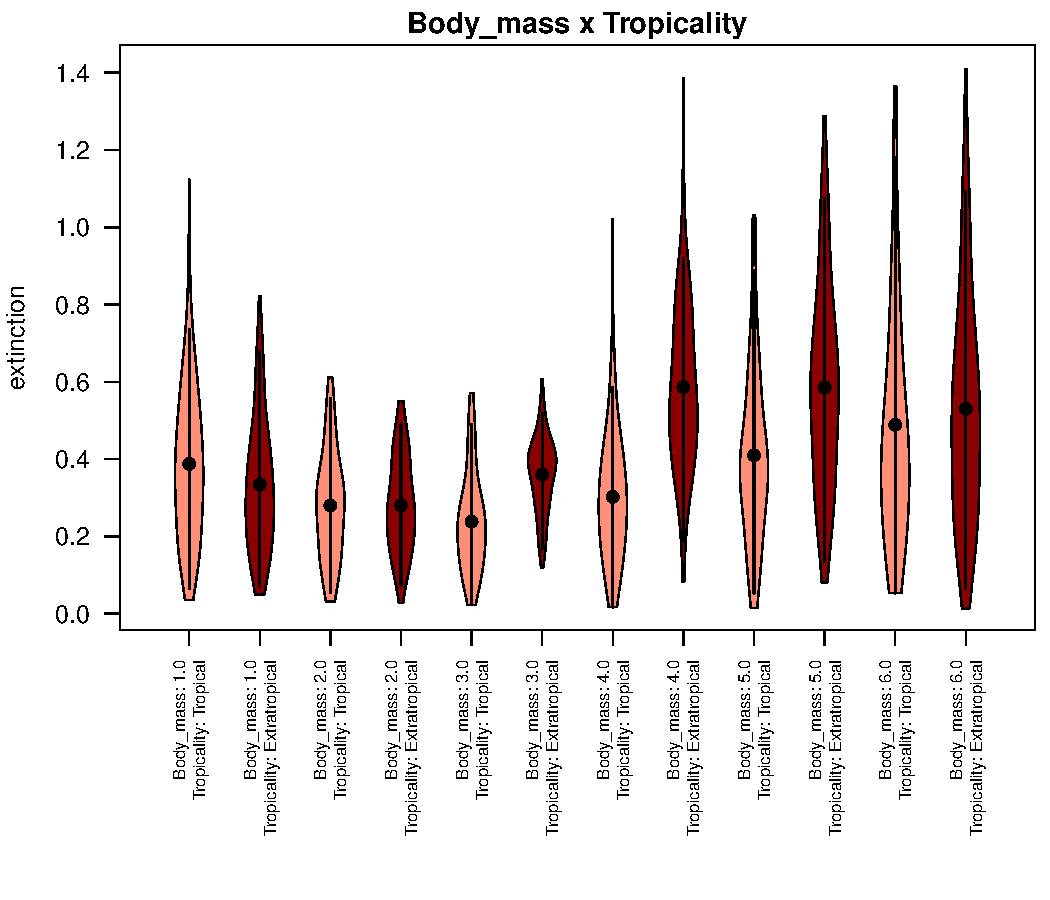
\includegraphics[width=13cm,height=\textheight]{../../Figures/Supp/Drivers_interaction/BM_Tropicality.pdf}

}

\caption{\label{fig-BMTrop}Interaction between latitude and body mass in
shaping chinchilloid extinction rate variations across lineages,
\emph{i}.\emph{e}., how sentitive to extinction body size classes are
with respect to their tropical (light red) or extratropical (dark red)
origin. Body mass categories are numbered from 1 to 6 by increasing
order (\emph{i}.\emph{e}., from XS to XXL). Results were arbitrarily
taken from the third imputation replicate of our BDNN analysis.}

\end{suppfigure}%

\begin{suppfigure}[H]

\centering{

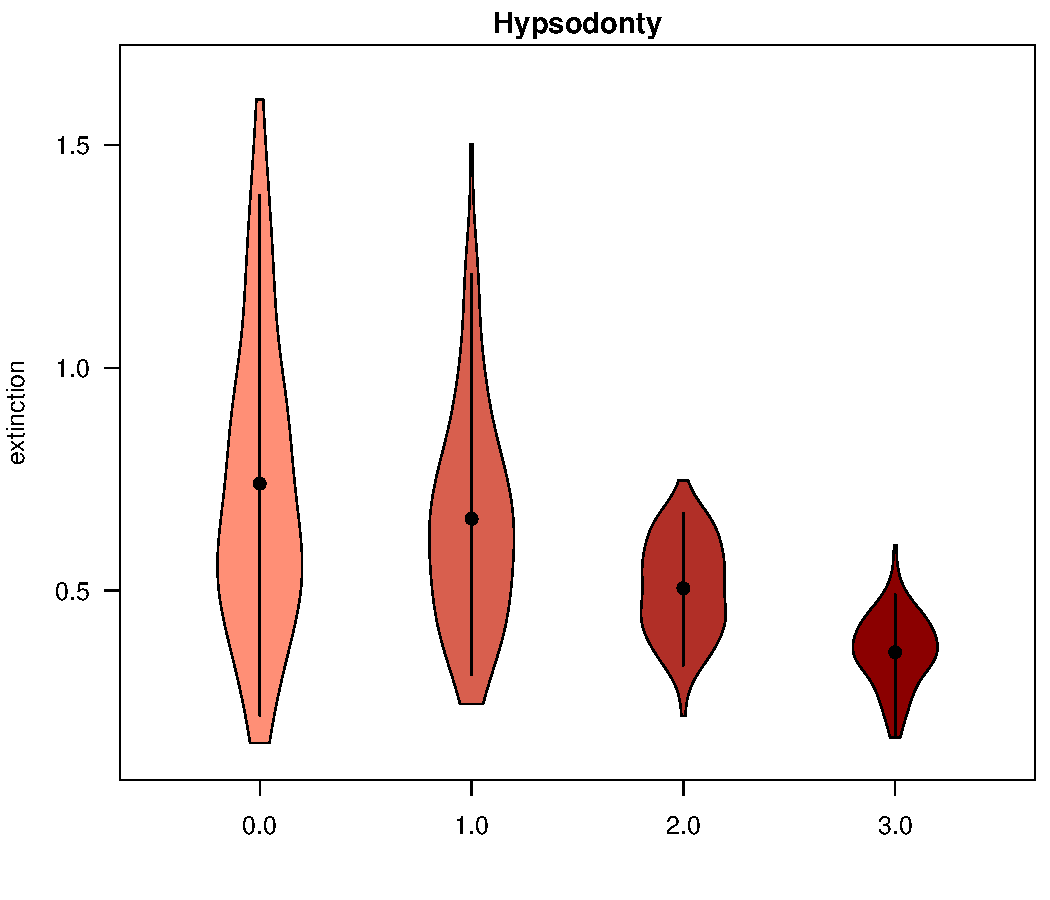
\includegraphics[width=13cm,height=\textheight]{../../Figures/Supp/Drivers_interaction/Hypsodonty.pdf}

}

\caption{\label{fig-hypso}How extinction rate varies across crown height
categories (0: brachydont, 1: mesodont, 2: protohypsodont and 3:
euhypsodont). Results were arbitrarily taken from the third imputation
replicate.}

\end{suppfigure}%

\newpage{}

\section{Supplementary Tables}\label{supplementary-tables}

\hfill\break

\begin{longtable}[]{@{}
  >{\centering\arraybackslash}p{(\columnwidth - 12\tabcolsep) * \real{0.1182}}
  >{\centering\arraybackslash}p{(\columnwidth - 12\tabcolsep) * \real{0.1545}}
  >{\centering\arraybackslash}p{(\columnwidth - 12\tabcolsep) * \real{0.0909}}
  >{\centering\arraybackslash}p{(\columnwidth - 12\tabcolsep) * \real{0.1909}}
  >{\centering\arraybackslash}p{(\columnwidth - 12\tabcolsep) * \real{0.1364}}
  >{\centering\arraybackslash}p{(\columnwidth - 12\tabcolsep) * \real{0.1545}}
  >{\centering\arraybackslash}p{(\columnwidth - 12\tabcolsep) * \real{0.1545}}@{}}

\caption{\label{tbl-DDperf}Performance of the different network
architectures tested in our DeepDive analyses. \texttt{LSTM\ Layers} and
\texttt{Fully-connected} are respectively the number of Long Short Term
Memory and Fully-connected units of the network (3: 128, 64 and 32
nodes; 2: 64 and 32 nodes; 1: 32 nodes). \texttt{Dropout} represents the
Monte-Carlo dropout fraction, that is, the proportion of connections
between neurons randomly toggled off between two learning epochs -- one
epoch being characterised by a complete pass through the entire training
dataset −, preventing from overfitting. \texttt{Nb.\ training\ epochs}
is the optimal number of training epochs. \texttt{Training\ loss} and
\texttt{Validation\ loss} are the values of the Mean Squared Error (MSE)
estimated between the `true' diversity of each simulated dataset (resp.
from the training or the validation set), and the predicted diversity
made by the network after \(n\) rounds of optimisation, where \(n\) is
the optimal number of training epochs. \texttt{Evaluation\ loss}
represent the MSE between each true and its associated predicted
diversity trajectory from the test datset, once the is trained
(\emph{i}.\emph{e}., after \(n\) rounds of optimisation, where \(n\) is
the optimal number of training epochs). The optimal number of epochs is
determined when the \texttt{Validation\ loss} starts increasing (see
Figure~S\ref{fig-ddHistPlotL2D2} and Figure~S\ref{fig-ddHistPlotL3D2}).
Architectures resulting in the smallest evaluation loss values,
\emph{i}.\emph{e}., generating the most accurate predictions, are
depicted in bold.}

\tabularnewline

\toprule\noalign{}
\begin{minipage}[b]{\linewidth}\centering
LSTM layers
\end{minipage} & \begin{minipage}[b]{\linewidth}\centering
Fully-connected
\end{minipage} & \begin{minipage}[b]{\linewidth}\centering
Dropout
\end{minipage} & \begin{minipage}[b]{\linewidth}\centering
Nb. training epochs
\end{minipage} & \begin{minipage}[b]{\linewidth}\centering
Training loss
\end{minipage} & \begin{minipage}[b]{\linewidth}\centering
Validation loss
\end{minipage} & \begin{minipage}[b]{\linewidth}\centering
Evaluation loss
\end{minipage} \\
\midrule\noalign{}
\endhead
\bottomrule\noalign{}
\endlastfoot
\textbf{3} & \textbf{2} & \textbf{0.05} & \textbf{16} & \textbf{0.314} &
\textbf{0.368} & \textbf{0.377} \\
3 & 1 & 0.05 & 14 & 0.324 & 0.367 & 0.38 \\
\textbf{2} & \textbf{2} & \textbf{0.05} & \textbf{22} & \textbf{0.349} &
\textbf{0.364} & \textbf{0.377} \\
2 & 1 & 0.05 & 19 & 0.354 & 0.366 & 0.38 \\
1 & 1 & 0.05 & 41 & 0.373 & 0.37 & 0.381 \\

\end{longtable}

\hfill\break

\begin{longtable}[]{@{}
  >{\raggedright\arraybackslash}p{(\columnwidth - 14\tabcolsep) * \real{0.0485}}
  >{\centering\arraybackslash}p{(\columnwidth - 14\tabcolsep) * \real{0.1515}}
  >{\centering\arraybackslash}p{(\columnwidth - 14\tabcolsep) * \real{0.1394}}
  >{\centering\arraybackslash}p{(\columnwidth - 14\tabcolsep) * \real{0.1273}}
  >{\centering\arraybackslash}p{(\columnwidth - 14\tabcolsep) * \real{0.1394}}
  >{\centering\arraybackslash}p{(\columnwidth - 14\tabcolsep) * \real{0.1273}}
  >{\centering\arraybackslash}p{(\columnwidth - 14\tabcolsep) * \real{0.1273}}
  >{\centering\arraybackslash}p{(\columnwidth - 14\tabcolsep) * \real{0.1394}}@{}}
\caption{Table representing the lower and upper bounds of the 95\% HPD
(resp. `q\_2.5\%' and `q\_97.5\%') of the distribution of the divergence
ages leading to all the extant chinchilloid species absent from the
fossil record -- \emph{i}.\emph{e}., all species but \emph{Lagostomus
maximus}. Ages are expressed in Ma.}\tabularnewline
\toprule\noalign{}
\begin{minipage}[b]{\linewidth}\raggedright
\end{minipage} & \begin{minipage}[b]{\linewidth}\centering
\emph{Chinchilla chinchilla}
\end{minipage} & \begin{minipage}[b]{\linewidth}\centering
\emph{Chinchilla lanigera}
\end{minipage} & \begin{minipage}[b]{\linewidth}\centering
\emph{Dinomys branickii}
\end{minipage} & \begin{minipage}[b]{\linewidth}\centering
\emph{Lagidium ahuacaense}
\end{minipage} & \begin{minipage}[b]{\linewidth}\centering
\emph{Lagidium peruanum}
\end{minipage} & \begin{minipage}[b]{\linewidth}\centering
\emph{Lagidium viscacia}
\end{minipage} & \begin{minipage}[b]{\linewidth}\centering
\emph{Lagidium wolffsohni}
\end{minipage} \\
\midrule\noalign{}
\endfirsthead
\toprule\noalign{}
\begin{minipage}[b]{\linewidth}\raggedright
\end{minipage} & \begin{minipage}[b]{\linewidth}\centering
\emph{Chinchilla chinchilla}
\end{minipage} & \begin{minipage}[b]{\linewidth}\centering
\emph{Chinchilla lanigera}
\end{minipage} & \begin{minipage}[b]{\linewidth}\centering
\emph{Dinomys branickii}
\end{minipage} & \begin{minipage}[b]{\linewidth}\centering
\emph{Lagidium ahuacaense}
\end{minipage} & \begin{minipage}[b]{\linewidth}\centering
\emph{Lagidium peruanum}
\end{minipage} & \begin{minipage}[b]{\linewidth}\centering
\emph{Lagidium viscacia}
\end{minipage} & \begin{minipage}[b]{\linewidth}\centering
\emph{Lagidium wolffsohni}
\end{minipage} \\
\midrule\noalign{}
\endhead
\bottomrule\noalign{}
\endlastfoot
q\_2.5\% & 0.78 & 0.78 & 16.54 & 2.20 & 1.34 & 0.56 & 0.56 \\
q\_97.5\% & 3.50 & 3.50 & 24.79 & 5.48 & 3.94 & 2.90 & 2.90 \\
\end{longtable}

\hfill\break

\begin{longtable}[]{@{}
  >{\centering\arraybackslash}p{(\columnwidth - 4\tabcolsep) * \real{0.3176}}
  >{\centering\arraybackslash}p{(\columnwidth - 4\tabcolsep) * \real{0.5176}}
  >{\centering\arraybackslash}p{(\columnwidth - 4\tabcolsep) * \real{0.1647}}@{}}

\caption{\label{tbl-Refsilhouettes}References of the silhouettes used in
Figure 1, from \href{https://www.phylopic.org/}{Phylopic}.}

\tabularnewline

\toprule\noalign{}
\begin{minipage}[b]{\linewidth}\centering
\textbf{Silhouette}
\end{minipage} & \begin{minipage}[b]{\linewidth}\centering
\textbf{Author}
\end{minipage} & \begin{minipage}[b]{\linewidth}\centering
\textbf{License}
\end{minipage} \\
\midrule\noalign{}
\endhead
\bottomrule\noalign{}
\endlastfoot
\emph{Chinchilla chinchilla} & Margot Michaud & CC0 1.0 \\
\emph{Lagidium peruanum} & Josue Hermoza & CC BY-SA 3.0 \\
\emph{Dinomys branickii} & Juan C. Cepeda Duque & CC BY 4.0 \\
\emph{Josephoartigasia monesi} & Nobu Tamura (body), Gustavo Lecuona
(head) & CC BY-SA 3.0 \\

\end{longtable}

\begin{longtable}[]{@{}ccc@{}}

\caption{\label{tbl-cv_sp}Coefficient of speciation rate variation
across the 10 BDNN replicates with random trait (\emph{i}.\emph{e}.,
body mass and/or hypsodonty index) imputation for taxa with missing
trait reconstruction (\(n=11\)), excluding Caribbean taxa. Simulated
values (\texttt{cv\_simulated}) were obtained from the analysis of 100
simulated datasets matching the empirical datasets in terms of number of
traits, clade age and (approximately) number of extant species,
generated under a constant-rate birth-death model. Empirical values
(\texttt{cv\_empirical}) were obtained from the analysis of the
empirical dataset. \emph{Note: significant variations of speciation rate
across lineages imply \texttt{cv\_empirical} \textgreater{}
\texttt{cv\_expected}}.}

\tabularnewline

\toprule\noalign{}
cv\_empirical & cv\_expected & Replicate \\
\midrule\noalign{}
\endhead
\bottomrule\noalign{}
\endlastfoot
0.22 & 0.21 & 1 \\
0.24 & 0.24 & 2 \\
0.26 & 0.22 & 3 \\
0.22 & 0.26 & 4 \\
0.22 & 0.23 & 5 \\
0.25 & 0.23 & 6 \\
0.2 & 0.2 & 7 \\
0.24 & 0.27 & 8 \\
0.27 & 0.2 & 9 \\
0.22 & 0.23 & 10 \\
\textbf{0.23} & \textbf{0.23} & \textbf{Mean} \\

\end{longtable}

\hfill\break

\begin{longtable}[]{@{}ccc@{}}

\caption{\label{tbl-cv_ex}Coefficient of extinction rate variation
across the 10 BDNN replicates with random trait (\emph{i}.\emph{e}.,
body mass and/or hypsodonty index) imputation for taxa with missing
trait reconstruction (\(n=11\)), excluding caribbean taxa. \emph{Note:
significant variations of speciation rate across lineages imply
\texttt{cv\_empirical} \textgreater{} \texttt{cv\_expected}}.}

\tabularnewline

\toprule\noalign{}
cv\_empirical & cv\_expected & Replicate \\
\midrule\noalign{}
\endhead
\bottomrule\noalign{}
\endlastfoot
0.49 & 0.33 & 1 \\
0.49 & 0.31 & 2 \\
0.46 & 0.33 & 3 \\
0.48 & 0.44 & 4 \\
0.44 & 0.47 & 5 \\
0.51 & 0.39 & 6 \\
0.47 & 0.34 & 7 \\
0.47 & 0.47 & 8 \\
0.5 & 0.26 & 9 \\
0.46 & 0.33 & 10 \\
\textbf{0.48} & \textbf{0.37} & \textbf{Mean} \\

\end{longtable}

\newpage{}

\begin{longtable}[]{@{}
  >{\centering\arraybackslash}p{(\columnwidth - 24\tabcolsep) * \real{0.1979}}
  >{\centering\arraybackslash}p{(\columnwidth - 24\tabcolsep) * \real{0.0625}}
  >{\centering\arraybackslash}p{(\columnwidth - 24\tabcolsep) * \real{0.0625}}
  >{\centering\arraybackslash}p{(\columnwidth - 24\tabcolsep) * \real{0.0625}}
  >{\centering\arraybackslash}p{(\columnwidth - 24\tabcolsep) * \real{0.0625}}
  >{\centering\arraybackslash}p{(\columnwidth - 24\tabcolsep) * \real{0.0625}}
  >{\centering\arraybackslash}p{(\columnwidth - 24\tabcolsep) * \real{0.0625}}
  >{\centering\arraybackslash}p{(\columnwidth - 24\tabcolsep) * \real{0.0625}}
  >{\centering\arraybackslash}p{(\columnwidth - 24\tabcolsep) * \real{0.0625}}
  >{\centering\arraybackslash}p{(\columnwidth - 24\tabcolsep) * \real{0.0625}}
  >{\centering\arraybackslash}p{(\columnwidth - 24\tabcolsep) * \real{0.0729}}
  >{\centering\arraybackslash}p{(\columnwidth - 24\tabcolsep) * \real{0.0938}}
  >{\centering\arraybackslash}p{(\columnwidth - 24\tabcolsep) * \real{0.0729}}@{}}

\caption{\label{tbl-pred_imp_ex}Predictor importance on extinction rate
across the 10 BDNN replicates with random trait (\emph{i}.\emph{e}.,
body mass and/or hypsodonty index) imputation for taxa with missing
trait reconstruction (\(n=11\)) after excluding caribbean taxa. We
highlighted in bold the three factors that contribute the most to
variations in extinction rates across species.}

\tabularnewline

\toprule\noalign{}
\begin{minipage}[b]{\linewidth}\centering
Predictor
\end{minipage} & \begin{minipage}[b]{\linewidth}\centering
R. 1
\end{minipage} & \begin{minipage}[b]{\linewidth}\centering
R. 2
\end{minipage} & \begin{minipage}[b]{\linewidth}\centering
R. 3
\end{minipage} & \begin{minipage}[b]{\linewidth}\centering
R. 4
\end{minipage} & \begin{minipage}[b]{\linewidth}\centering
R. 5
\end{minipage} & \begin{minipage}[b]{\linewidth}\centering
R. 6
\end{minipage} & \begin{minipage}[b]{\linewidth}\centering
R. 7
\end{minipage} & \begin{minipage}[b]{\linewidth}\centering
R. 8
\end{minipage} & \begin{minipage}[b]{\linewidth}\centering
R. 9
\end{minipage} & \begin{minipage}[b]{\linewidth}\centering
R. 10
\end{minipage} & \begin{minipage}[b]{\linewidth}\centering
SumRank
\end{minipage} & \begin{minipage}[b]{\linewidth}\centering
Rank
\end{minipage} \\
\midrule\noalign{}
\endhead
\bottomrule\noalign{}
\endlastfoot
\textbf{Andean\_uplift} & 1 & 1 & 1 & 1 & 1 & 1 & 1 & 1 & 1 & 1 & 10 &
\textbf{1} \\
\textbf{Body\_mass} & 2 & 2 & 2 & 2 & 2 & 2 & 2 & 2 & 2 & 2 & 20 &
\textbf{2} \\
\textbf{Tropicality} & 4 & 4 & 3 & 3 & 4 & 3 & 3 & 4 & 4 & 3 & 35 &
\textbf{3} \\
Crown\_Height & 3 & 3 & 5 & 4 & 3 & 5 & 5 & 3 & 3 & 4 & 38 & 4 \\
Self\_diversity & 5 & 5 & 4 & 4 & 5 & 4 & 4 & 5 & 5 & 5 & 46 & 5 \\
Temperature & 6 & 7 & 6 & 5 & 7 & 6 & 7 & 6 & 6 & 6 & 62 & 6 \\
Sea\_level & 7 & 6 & 7 & 7 & 6 & 7 & 6 & 7 & 7 & 7 & 67 & 7 \\
time & 8 & 8 & 8 & 8 & 8 & 8 & 8 & 8 & 8 & 8 & 80 & 8 \\

\end{longtable}

\begin{longtable}[]{@{}cccc@{}}

\caption{\label{tbl-FC_BM}Magnitude of the change in extinction rate
(\emph{i}.\emph{e}., \texttt{Fold\ Change}) between the two extreme body
size classes showing the most pronounced extinction rate variation (S
and XL; Figure 6A) across the 10 trait-imputed replicates without
Caribbean taxa. \texttt{Upper\ CI} and \texttt{Lower\ CI} respectively
show the uppper and lower boundaries of the associated 95\% HPD
interval. The `Total' row shows the averaged values across the 10
replicates.}

\tabularnewline

\toprule\noalign{}
Replicate & Fold Change & Upper CI & Lower CI \\
\midrule\noalign{}
\endhead
\bottomrule\noalign{}
\endlastfoot
1 & 1.6 & 5.99 & -2.77 \\
2 & 1.94 & 7.17 & -2.49 \\
3 & 2.3 & 7.25 & -1.69 \\
4 & 1.89 & 6.51 & -2.09 \\
5 & 1.85 & 5.53 & -1.78 \\
6 & 1.65 & 8.96 & -3.48 \\
7 & 1.68 & 5.16 & -2.48 \\
8 & 1.75 & 6.26 & -2.46 \\
9 & 1.9 & 6.77 & -2.64 \\
10 & 1.8 & 6.62 & -2.65 \\
\textbf{Mean} & \textbf{1.84} & \textbf{6.62} & \textbf{-2.46} \\

\end{longtable}

\begin{longtable}[]{@{}cccc@{}}

\caption{\label{tbl-FC_ET}Magnitude of the change in extinction rate
(\emph{i}.\emph{e}., fold change) between tropical and extratropical
taxa across the 10 trait-imputated replicates without Caribbean taxa.
\texttt{Upper\ CI} and \texttt{Lower\ CI} respectively show the uppper
and lower boundaries of the associated 95\% HPD interval. The `Total'
row shows the averaged values across the 10 replicates.}

\tabularnewline

\toprule\noalign{}
Replicate & Fold Change & Upper CI & Lower CI \\
\midrule\noalign{}
\endhead
\bottomrule\noalign{}
\endlastfoot
1 & 1.59 & 4.72 & -1.51 \\
2 & 1.53 & 4.77 & -1.47 \\
3 & 1.42 & 3.55 & -1.44 \\
4 & 1.36 & 4.04 & -1.79 \\
5 & 1.52 & 3.81 & -1.56 \\
6 & 1.52 & 5.16 & -1.93 \\
7 & 1.48 & 3.85 & -1.58 \\
8 & 1.49 & 4.07 & -1.38 \\
9 & 1.59 & 4.49 & -1.69 \\
10 & 1.46 & 3.86 & -1.78 \\
\textbf{Mean} & \textbf{1.5} & \textbf{4.23} & \textbf{-1.61} \\

\end{longtable}

\begin{longtable}[]{@{}cccc@{}}

\caption{\label{tbl-FC_hypso}Magnitude of the change in extinction rate
(\emph{i}.\emph{e}., fold change) between protohypsodont and euhypsodont
taxa across the 10 trait-imputated replicates without Caribbean taxa.
\texttt{Upper\ CI} and \texttt{Lower\ CI} respectively show the uppper
and lower boundaries of the associated 95\% HPD interval. The `Total'
row shows the averaged values across the 10 replicates.}

\tabularnewline

\toprule\noalign{}
Replicate & Fold Change & Upper CI & Lower CI \\
\midrule\noalign{}
\endhead
\bottomrule\noalign{}
\endlastfoot
1 & -1.74 & -1 & -4.96 \\
2 & -1.65 & 1.26 & -3.66 \\
3 & -1.43 & 1.47 & -2.75 \\
4 & -1.42 & 1.54 & -2.94 \\
5 & -1.53 & 1.32 & -2.87 \\
6 & -1.53 & 1.41 & -3.17 \\
7 & -1.49 & 1.35 & -2.9 \\
8 & -1.66 & 1.25 & -3.53 \\
9 & -1.63 & 1.28 & -3.6 \\
10 & -1.49 & 1.28 & -2.95 \\
\textbf{Mean} & \textbf{-1.56} & \textbf{1.12} & \textbf{-3.33} \\

\end{longtable}

\begin{longtable}[]{@{}ccc@{}}

\caption{\label{tbl-MBDex}Posterior estimates of the multivariate
birth--death (MBD) correlation parameters with the extinction rate
(\(G_{\mu}\), median), shown along with their 95\% Highest Posterior
Density (HPD) interval, for each of the four environmental variable
tested. The only significant correlation, \emph{i}.\emph{e}., of which
the 95\% HPD of the associated coefficient does not significantly
overlap with 0, is shown in bold.}

\tabularnewline

\toprule\noalign{}
Covar & G\_mu & G\_mu\_95HPD \\
\midrule\noalign{}
\endhead
\bottomrule\noalign{}
\endlastfoot
Self-diversity & 0.81 & {[}-0.25; 2.02{]} \\
Regional Temperature & 0 & {[}-0.22; 0.21{]} \\
Andes Elevation & 0.07 & {[}-0.18; 0.29{]} \\
\textbf{Sea Level} & \textbf{0.21} & \textbf{{[}0; 0.46{]}} \\

\end{longtable}

\begin{longtable}[]{@{}ccc@{}}

\caption{\label{tbl-MBDsp}Posterior estimates of the multivariate
birth--death (MBD) correlation parameters with the speciation rate
(\(G_{\mu}\), median), shown along with their 95\% Highest Posterior
Density (HPD) interval, for each of the four environmental variable
tested. As all HPD intervals overlap with zero, no ignificant
correlation was highlighted by this analysis.}

\tabularnewline

\toprule\noalign{}
Covar & G\_lamb & G\_lamb\_95HPD \\
\midrule\noalign{}
\endhead
\bottomrule\noalign{}
\endlastfoot
Self-diversity & -0.41 & {[}-1.58; 0.58{]} \\
Regional Temperature & 0.09 & {[}-0.11; 0.35{]} \\
Andes Elevation & 0.06 & {[}-0.16; 0.31{]} \\
Sea Level & -0.07 & {[}-0.29; 0.13{]} \\

\end{longtable}

\begin{longtable}[]{@{}ccc@{}}

\caption{\label{tbl-ADEcoeff}Median estimate and associated 95\% HPD
bounds of the shape parameter of the Weibull shape parameter (\(\Phi\))
of the Age-Dependent Extinction analysis of our species-level
chinchilloid temporal occurrence dataset. Since the ADE model should be
run on periods of constant extinction rate through time,
\texttt{Species\_Early} and \texttt{Species\_After} respectively
designate the species before and after the shift in extinction rate
occurring \emph{ca}. 6 Ma.}

\tabularnewline

\toprule\noalign{}
Phase & Median\_estimate & HPD95 \\
\midrule\noalign{}
\endhead
\bottomrule\noalign{}
\endlastfoot
Species Early & 0.66 & {[}0.4; 0.99{]} \\
Species Late & 0.36 & {[}0.21; 0.65{]} \\

\end{longtable}

\newpage{}

\section{Supplementary references}\label{supplementary-references}

\phantomsection\label{refs}
\begin{CSLReferences}{1}{1}
\bibitem[\citeproctext]{ref-arnal2026}
Arnal M., Kay R.F., Valdivia L.A., Salenbien W., Morse P.E., Borths
M.R., Williams B.A., Riddle C., Martínez J.-N., Gonzales L.A. 2026.
\href{https://doi.org/10.1002/spp2.70064}{New Early Miocene
hystricognath rodents (Caviomorpha) from the Madre de Dios River in the
southeastern Peruvian Amazon}. Papers in Palaeontology. 12:e70064.

\bibitem[\citeproctext]{ref-arnal2019}
Arnal M., Pérez M.E., Deschamps C. 2019.
\href{https://doi.org/10.5710/PEAPA.25.09.2019.299}{Revision of the
Miocene Caviomorph Rodents From the Río Santa Cruz (Argentinean
Patagonia)}. Publicación Electrónica de la Asociación Paleontológica
Argentina. 19.

\bibitem[\citeproctext]{ref-boivin2019}
Boivin M., Marivaux L., Antoine P.-O. 2019.
\href{https://doi.org/10.5252/geodiversitas2019v41a4}{L'apport du
registre paléogène d'amazonie sur la diversification initiale des
caviomorpha (hystricognathi, rodentia): Implications phylogénétiques,
macroévolutives et paléobiogéographiques}. Geodiversitas. 41:143--245.

\bibitem[\citeproctext]{ref-boschman2021}
Boschman L.M. 2021.
\href{https://doi.org/10.1016/j.earscirev.2021.103640}{Andean mountain
building since the late cretaceous: A paleoelevation reconstruction}.
Earth-Science Reviews. 220:103640.

\bibitem[\citeproctext]{ref-bostelmann2013}
Bostelmann J.E., Roux J.P.L., Vásquez A., Gutiérrez N.M., Oyarzún J.L.,
Carreño C., Torres T., Otero R., Llanos A., Fanning C.M., Hervé F. 2013.
\href{https://doi.org/10.5027/andgeoV40n3-a04}{Burdigalian deposits of
the Santa Cruz Formation in the Sierra Baguales, Austral (Magallanes)
Basin: Age, depositional environment and vertebrate fossils}. Andean
Geology. 40:458--489.

\bibitem[\citeproctext]{ref-brandoni2016}
Brandoni D., Ruiz L.G., Tejedor M.F., Martin G., Fleagle J.G. 2016.
\href{https://doi.org/10.1007/s12542-016-0306-8}{Megatherioidea
(Mammalia, Xenarthra, Tardigrada) from the Pinturas Formation (Early
Miocene), Santa Cruz Province (Argentina) and their chronological
implications}. PalZ. 90:619--628.

\bibitem[\citeproctext]{ref-bucher2021}
Bucher J., Pérez M.E., González Ruiz L.R., D'Elía L., Bilmes A. 2021.
\href{https://doi.org/10.1016/j.jsames.2020.103024}{New middle miocene
(langhian - serravallian) vertebrate localities in northwestern
patagonia, argentina: A contribution to high latitude south american
land mammal ages sequence}. Journal of South American Earth Sciences.
107:103024.

\bibitem[\citeproctext]{ref-burgin2025}
Burgin C.J., Zijlstra J.S., Becker M.A., Handika H., Alston J.M.,
Widness J., Liphardt S., Huckaby D.G., Upham N.S. 2025.
\href{https://doi.org/10.1101/2025.02.27.640393}{{H}ow many mammal
species are there now? {U}pdates and trends in taxonomic, nomenclatural,
and geographic knowledge}.

\bibitem[\citeproctext]{ref-busker2019}
Busker F., Pérez M.E., Dozo M.T. 2019.
\href{https://doi.org/10.1016/j.crpv.2019.05.003}{A new chinchilloid
(rodentia, hystricognathi) from the early miocene of the localities of
bryn gwyn and gran barranca (patagonia, argentina)}. Comptes Rendus
Palevol. 18:525--540.

\bibitem[\citeproctext]{ref-carrillo2026}
Carrillo J.D., Torres Jimenez M.F., Urrea-Barreto F.J., Pino K., Cooper
R.B., Antonelli A., Bacon C.D., Faurby S., Silvestro D. 2026.
\href{https://doi.org/10.1098/rspb.2025.2586}{Decoupled diversity and
disparity after faunistic turnover in caviomorph rodents}. Proceedings
of the Royal Society B: Biological Sciences. 293:20252586.

\bibitem[\citeproctext]{ref-dacunha2023}
Da Cunha L., Viñola-López L.W., MacPhee R.D.E., Kerber L., Vélez-Juarbe
J., Antoine P.-O., Boivin M., Hautier L., Lebrun R., Marivaux L., Fabre
P.-H. 2023. \href{https://doi.org/10.1007/s10914-023-09675-3}{{T}he
inner ear of caviomorph rodents: {P}hylogenetic implications and
application to extinct {W}est {I}ndian taxa}. Journal of Mammalian
Evolution. 30:1155--1176.

\bibitem[\citeproctext]{ref-esteban2019}
Esteban G.I., Georgieff S.M., Nasif N.L., Ibáñez L., Bonini R.A. 2019.
Marco estratigráfico, paleontología de vertebrados y paleoambientes del
plioceno de catamarca, tucumán y santiago del estero, argentina. p.
348--366.

\bibitem[\citeproctext]{ref-esteban2014}
Esteban G.I., Nasif N.L., Georgieff S.M. 2014. Cronobioestratigrafia del
mioceno tardio-plioceno temprano, puerta de corral quemado y villavil,
provincia de catamarca, argentina. Acta geológica lilloan. 26:165--192.

\bibitem[\citeproctext]{ref-fernicola2019}
Fernicola J.C., Vizcaíno S.F., Bargo M.S., Kay R.F., Cuitiño J.I. 2019.
\href{https://doi.org/10.5710/PEAPA.01.11.2019.309}{Analysis of the
Early{\textendash}Middle Miocene mammal associations at the río Santa
Cruz (Patagonia, Argentina)}. Publicación Electrónica de la Asociación
Paleontológica Argentina. 19.

\bibitem[\citeproctext]{ref-kramarz2002}
Kramarz A. 2002.
\href{https://revista.macn.gob.ar/index.php/RevMus/article/view/9}{Roedores
chinchilloideos (Hystricognathi) de la Formación Pinturas, Mioceno
temprano-medio de la provincia de Santa Cruz, Argentina}. Revista del
Museo Argentino de Ciencias Naturales nueva serie. 4:167--180.

\bibitem[\citeproctext]{ref-kramarz2004}
Kramarz A.G. 2004.
\href{https://www.ameghiniana.org.ar/index.php/ameghiniana/article/view/815}{Octodontoids
and erethizontoids (Rodentia, Hystricognathi) from the Pinturas
Formation, Early - Middle Miocene of Patagonia, Argentina}. Ameghiniana.
41:199--216.

\bibitem[\citeproctext]{ref-kramarz2006}
Kramarz A.G. 2006.
\href{https://www.jstor.org/stable/4524620}{Eocardiids (rodentia,
hystricognathi) from the pinturas formation, late early miocene of
patagonia, argentina}. Journal of Vertebrate Paleontology. 26:770--778.

\bibitem[\citeproctext]{ref-macphee2011}
MacPhee R.D.E. 2011.
\href{https://doi.org/10.1206/0003-0090-363.1.1}{{B}asicranial
{M}orphology and {R}elationships of {A}ntillean {H}eptaxodontidae
({R}odentia, {C}tenohystrica, {C}aviomorpha)}. Bulletin of the American
Museum of Natural History. 2011:1--70.

\bibitem[\citeproctext]{ref-marivaux2022}
Marivaux L., López L.W.V., Boivin M., Da Cunha L., Fabre P.-H.,
Joannes-Boyau R., Maincent G., Münch P., Stutz N.S., Vélez-Juarbe J.,
Antoine P.-O. 2022.
\href{https://doi.org/10.1007/s10914-022-09631-7}{{I}ncisor enamel
microstructure of {W}est {I}ndian caviomorph hystricognathous rodents
({O}ctodontoidea and {C}hinchilloidea)}. Journal of Mammalian Evolution.
29:969--995.

\bibitem[\citeproctext]{ref-marivaux_early_2020}
Marivaux L., Vélez-Juarbe J., Merzeraud G., Pujos F., Viñola López L.W.,
Boivin M., Santos-Mercado H., Cruz E.J., Grajales A., Padilla J.,
Vélez-Rosado K.I., Philippon M., Léticée J.-L., Münch P., Antoine P.-O.
2020. \href{https://doi.org/10.1098/rspb.2019.2806}{Early oligocene
chinchilloid caviomorphs from puerto rico and the initial rodent
colonization of the west indies}. Proceedings of the Royal Society B:
Biological Sciences. 287:20192806.

\bibitem[\citeproctext]{ref-miller2020}
Miller K.G., Browning J.V., Schmelz W.J., Kopp R.E., Mountain G.S.,
Wright J.D. 2020. \href{https://doi.org/10.1126/sciadv.aaz1346}{Cenozoic
sea-level and cryospheric evolution from deep-sea geochemical and
continental margin records}. Science Advances. 6:eaaz1346.

\bibitem[\citeproctext]{ref-rasia2016}
Rasia L.L. 2016. \href{https://doi.org/10.35537/10915/54323}{Los
Chinchillidae (Rodentia,Caviomorpha) fósiles de la República Argentina:
sistemática, historia evolutiva y biogeográfica, significado
bioestratigráfico y paleoambiental}.

\bibitem[\citeproctext]{ref-rasia_vizcacha_2024}
Rasia L.L. 2024.
\href{https://doi.org/10.1007/978-3-031-49487-1_3}{Fossil record of
lagostomus: A 10 million years story}. In: Rasia L.L., Barbeito C.G.,
Acuña F., editors. Plains vizcachas: Biology and evolution of a peculiar
neotropical caviomorph rodent. Cham: Springer Nature Switzerland. p.
27--42.

\bibitem[\citeproctext]{ref-rasia2026}
Rasia L.L. 2026. Reassessing the hyperdiverse dinomyid (rodentia,
caviomorpha) assemblage from the late miocene ituzaingó formation (entre
ríos province, argentina). Ameghiniana.

\bibitem[\citeproctext]{ref-rasia2012}
Rasia L.L., Candela A.M. 2012.
\href{https://doi.org/10.4202/app.2011.0041}{Systematic and
biostratigraphic significance of a chinchillid rodent from the pliocene
of eastern argentina}. Acta Palaeontologica Polonica. 58:241--254.

\bibitem[\citeproctext]{ref-rasia_comprehensive_2021}
Rasia L.L., Candela A.M., Cañón C. 2021.
\href{https://doi.org/10.1111/joa.13430}{Comprehensive total evidence
phylogeny of chinchillids (rodentia, caviomorpha): Cheek teeth anatomy
and evolution}. Journal of Anatomy. 239:405--423.

\bibitem[\citeproctext]{ref-romano2023}
Romano C.O., Garrido A.C., Barbeau Jr D.L., Vera R.B., Bonini R.,
Boscaini A., Cerdeño E., Cruz L.E., Esteban G.I., Fuente M.S. de la,
Fernández-Monescillo M., Fernicola J.C., Krapovickas V., Madozzo-Jaén
M.C., Pérez M.E., Pujos F., Rasia L., Turazzini G.F., Vera B., MacPhee
R.D.E., Forasiepi A.M., Prevosti F.J. 2023.
\href{https://doi.org/10.1002/spp2.1539}{Redefining the Huayquerian
Stage (Upper Miocene to Lower Pliocene) of the South American
chronostratigraphic scale based on biostratigraphical analyses and
geochronological dating}. Papers in Palaeontology. 9:e1539.

\bibitem[\citeproctext]{ref-tardif2025}
Tardif D., Condamine F.L., Streiff S.J.R., Sepulchre P., Couvreur T.L.P.
2025. \href{https://doi.org/10.1111/geb.70024}{Generating Spatialised
and Seasonal Deep-Time Palaeoclimatic Information: Integration Into an
Environmental-Dependent Diversification Model}. Global Ecology and
Biogeography. 34:e70024.

\bibitem[\citeproctext]{ref-ubilla2016}
Ubilla M., Rinderknecht A. 2016.
\href{https://doi.org/10.1080/03115518.2016.1145466}{Lagostomus maximus
(desmarest) (rodentia, chinchillidae), the extant plains vizcacha in the
late pleistocene of uruguay}. Alcheringa: An Australasian Journal of
Palaeontology. 40:354--365.

\bibitem[\citeproctext]{ref-vizcaino2022}
Vizcaino S.F., Bargo M.S., Pérez M.E., Aramendía I., Cuitiño J.I.,
Monsalvo E.S., Vlachos E., Noriega J.I., Kay R.F. 2022.
\href{https://doi.org/10.5027/andgeoV49n3-3425}{Fossil vertebrates of
the early-middle Miocene Cerro Boleadoras Formation, northwestern Santa
Cruz Province, Patagonia, Argentina}. Andean Geology. 49:382--422.

\bibitem[\citeproctext]{ref-woods2021}
Woods R., Barnes I., Brace S., Turvey S.T. 2021.
\href{https://doi.org/10.1093/molbev/msaa189}{{A}ncient {D}{N}{A}
{S}uggests {S}ingle {C}olonization and {W}ithin-{A}rchipelago
{D}iversification of {C}aribbean {C}aviomorph {R}odents}. Molecular
Biology and Evolution. 38:84--95.

\end{CSLReferences}




\end{document}
